% This file was converted to LaTeX by Writer2LaTeX ver. 1.2
% see http://writer2latex.sourceforge.net for more info
\documentclass[twoside,letterpaper]{article}
\usepackage[ascii]{inputenc}
\usepackage[T1]{fontenc}
\usepackage[english]{babel}
\usepackage{amsmath}
\usepackage{amssymb,amsfonts,textcomp}
\usepackage{color}
\usepackage{array}
\usepackage{supertabular}
\usepackage{hhline}
\usepackage{hyperref}
\hypersetup{pdftex, colorlinks=true, linkcolor=black, citecolor=black, filecolor=black, urlcolor=black, pdftitle=SYSTEMS AND SOFTWARE REQUIREMENTS SPECIFICATION (SSRS) TEMPLATE, pdfauthor=Clinton Jeffery, pdfsubject=, pdfkeywords=}
\usepackage[pdftex]{graphicx}
%\graphicspath{ {images/} }
% footnotes configuration
\makeatletter
\renewcommand\thefootnote{\arabic{footnote}}
\makeatother
% Outline numbering
\setcounter{secnumdepth}{3}
\renewcommand\thesection{\arabic{section}}
\renewcommand\thesubsection{\arabic{section}.\arabic{subsection}}
\renewcommand\thesubsubsection{\arabic{section}.\arabic{subsection}.\arabic{subsubsection}}
\renewcommand\thesubparagraph{\arabic{section}.\arabic{subsection}.\arabic{subsubsection}.null{paragraph}.\arabic{subparagraph}}
\makeatletter
\newcommand\arraybslash{\let\\\@arraycr}
\makeatother
% Page layout (geometry)
\setlength\voffset{-1in}
\setlength\hoffset{-1in}
\setlength\topmargin{0.5in}
\setlength\oddsidemargin{1in}
\setlength\evensidemargin{1in}
\setlength\textheight{8.278in}
\setlength\textwidth{6.5in}
\setlength\footskip{0.561in}
\setlength\headheight{0.5in}
\setlength\headsep{0.461in}
% Footnote rule
\setlength{\skip\footins}{0.0469in}
\renewcommand\footnoterule{\vspace*{-0.0071in}\setlength\leftskip{0pt}\setlength\rightskip{0pt plus 1fil}\noindent\textcolor{black}{\rule{0.25\columnwidth}{0.0071in}}\vspace*{0.0398in}}
% Pages styles
\makeatletter
\newcommand\ps@Standard{
  \renewcommand\@oddhead{\rmfamily\color{black} University of Idaho CS Department Instructional Use\hfill \hfill NOT FOR RELEASE}
  \renewcommand\@evenhead{\@oddhead}
  \renewcommand\@oddfoot{{\foreignlanguage{english}{\textcolor{black}{SSRS Page }}}{\foreignlanguage{english}{\textcolor{black}{\thepage{}}}}}
  \renewcommand\@evenfoot{\@oddfoot}
  \renewcommand\thepage{\arabic{page}}
}
\newcommand\ps@Convertviii{
  \renewcommand\@oddhead{\selectlanguage{english}\rmfamily\color{black} University of Idaho CS Department Instructional Use\hfill \hfill NOT FOR RELEASE}
  \renewcommand\@evenhead{\@oddhead}
  \renewcommand\@oddfoot{{\foreignlanguage{english}{\textcolor{black}{SSRS Page }}}{\foreignlanguage{english}{\textcolor{black}{\thepage{}}}}}
  \renewcommand\@evenfoot{\@oddfoot}
  \renewcommand\thepage{\arabic{page}}
}
\newcommand\ps@Convertvii{
  \renewcommand\@oddhead{\selectlanguage{english}\rmfamily\color{black} University of Idaho CS Department Instructional Use\hfill \hfill NOT FOR RELEASE}
  \renewcommand\@evenhead{\@oddhead}
  \renewcommand\@oddfoot{{\foreignlanguage{english}{\textcolor{black}{SSRS Page }}}{\foreignlanguage{english}{\textcolor{black}{\thepage{}}}}}
  \renewcommand\@evenfoot{\@oddfoot}
  \renewcommand\thepage{\arabic{page}}
}
\newcommand\ps@Convertvi{
  \renewcommand\@oddhead{\selectlanguage{english}\rmfamily\color{black} University of Idaho CS Department Instructional Use\hfill \hfill \hfill \hfill  \ \ \ \ \ NOT FOR RELEASE}
  \renewcommand\@evenhead{\@oddhead}
  \renewcommand\@oddfoot{{\foreignlanguage{english}{\textcolor{black}{SSRS Page }}}{\foreignlanguage{english}{\textcolor{black}{\thepage{}}}}}
  \renewcommand\@evenfoot{\@oddfoot}
  \renewcommand\thepage{\arabic{page}}
}
\newcommand\ps@Convertv{
  \renewcommand\@oddhead{\selectlanguage{english}\rmfamily\color{black} University of Idaho CS Department Instructional Use\hfill \hfill NOT FOR RELEASE}
  \renewcommand\@evenhead{\@oddhead}
  \renewcommand\@oddfoot{{\foreignlanguage{english}{\textcolor{black}{SSRS Page }}}{\foreignlanguage{english}{\textcolor{black}{\thepage{}}}}}
  \renewcommand\@evenfoot{\@oddfoot}
  \renewcommand\thepage{\arabic{page}}
}
\newcommand\ps@Convertiv{
  \renewcommand\@oddhead{\selectlanguage{english}\rmfamily\color{black} University of Idaho CS Department Instructional Use\hfill \hfill \hfill \hfill  \ \ \ \ \ \ NOT FOR RELEASE}
  \renewcommand\@evenhead{\@oddhead}
  \renewcommand\@oddfoot{{\foreignlanguage{english}{\textcolor{black}{SSRS Page }}}{\foreignlanguage{english}{\textcolor{black}{\thepage{}}}}}
  \renewcommand\@evenfoot{\@oddfoot}
  \renewcommand\thepage{\arabic{page}}
}
\newcommand\ps@Convertii{
  \renewcommand\@oddhead{}
  \renewcommand\@evenhead{\@oddhead}
  \renewcommand\@oddfoot{}
  \renewcommand\@evenfoot{\@oddfoot}
  \renewcommand\thepage{\arabic{page}}
}
\makeatother
\pagestyle{Standard}
\setlength\tabcolsep{1mm}
\renewcommand\arraystretch{1.3}
\title{SYSTEMS AND SOFTWARE REQUIREMENTS SPECIFICATION (SSRS) TEMPLATE}
\author{Clinton Jeffery}
\date{2013-09-10}
\begin{document}
\clearpage\setcounter{page}{1}\pagestyle{Standard}


\clearpage{\centering\bfseries
SYSTEMS AND SOFTWARE \ REQUIREMENTS SPECIFICATION (SSRS) FOR
\par}


\bigskip

{\centering\bfseries
sQuire Collaborative IDE
\par}


\bigskip


\bigskip


\bigskip

\begin{center}
Picture here.
\end{center}

\bigskip


\bigskip

{\centering\bfseries
Version 1.0
\par}

{\centering\bfseries
February 09, 2016
\par}


\bigskip


\bigskip

{\centering\bfseries
Prepared for:
\par}

{\centering\bfseries
CS383-01
\par}


\bigskip


\bigskip

{\centering\bfseries
Prepared by:
\par}

{\centering\bfseries
Domn Werner (wern0096) $\vert$ Robert Carlson (carl7595) $\vert$ Brian Cartwright (cart1189) \\ Max Welch (welc2150) $\vert$ Matthew Daniel (dani2918) $\vert$ Brandon Ratcliff (ratc8795) \\ Joel Doumit (doum6708) $\vert$ Eric Gentile-Quant (gent7104) \\
Team 4 - It Compiled Yesterday (ICY)
\par}

{\centering\bfseries
University of Idaho
\par}

{\centering\bfseries
Moscow, ID \ 83844-1010
\par}

\clearpage{\centering\bfseries
sQuire SSRS
\par}


\bigskip

{\centering\bfseries
RECORD OF CHANGES
\par}


\bigskip

\begin{flushleft}
\tablefirsthead{}
\tablehead{}
\tabletail{}
\tablelasttail{}
\begin{supertabular}{|m{0.47685984in}|m{0.6087598in}|m{1.3587599in}|m{0.23375985in}|m{2.0462599in}|m{0.7337598in}|m{0.6330598in}|}
\hline
~

\centering{\selectlanguage{english}\color{black} Change number} &
~

\centering{\selectlanguage{english}\color{black} Date completed} &
~

\centering{\selectlanguage{english}\color{black} Location of change (e.g., page or figure \#)} &
\centering{\selectlanguage{english}\bfseries\color{black} A\newline
M\newline
D} &
~

~

\centering{\selectlanguage{english}\color{black} Brief description of change} &
~

\centering{\selectlanguage{english}\color{black} Approved by (initials)} &
~

\centering\arraybslash{\selectlanguage{english}\color{black} Date Approved}\\\hline
1 & 02/11/16 & Page 1 & M & Updated Team Name & DW & 02/11/16 \\\hline
2 & 02/11/16 & Pages 8-10 & M & Updated Functional Reqs & DW & 02/11/16\\\hline
3 & 02/18/16 & Section 3.3 & A & Added Use Cases & DW & 02/18/16 \\\hline
4 & 02/18/16 & Section 3.4  & A & Added Class Diagram Section & DW & 02/18/16 \\\hline
5 & 03/02/16 & Section 3.3 & M & Included Sequence Diagrams & DW & 03/02/16 \\\hline
~
 &
~
 &
~
 &
~
 &
~
 &
~
 &
~
\\\hline
~
 &
~
 &
~
 &
~
 &
~
 &
~
 &
~
\\\hline
~
 &
~
 &
~
 &
~
 &
~
 &
~
 &
~
\\\hline
~
 &
~
 &
~
 &
~
 &
~
 &
~
 &
~
\\\hline
~
 &
~
 &
~
 &
~
 &
~
 &
~
 &
~
\\\hline
~
 &
~
 &
~
 &
~
 &
~
 &
~
 &
~
\\\hline
~
 &
~
 &
~
 &
~
 &
~
 &
~
 &
~
\\\hline
~
 &
~
 &
~
 &
~
 &
~
 &
~
 &
~
\\\hline
~
 &
~
 &
~
 &
~
 &
~
 &
~
 &
~
\\\hline
~
 &
~
 &
~
 &
~
 &
~
 &
~
 &
~
\\\hline
~
 &
~
 &
~
 &
~
 &
~
 &
~
 &
~
\\\hline
~
 &
~
 &
~
 &
~
 &
~
 &
~
 &
~
\\\hline
~
 &
~
 &
~
 &
~
 &
~
 &
~
 &
~
\\\hline
~
 &
~
 &
~
 &
~
 &
~
 &
~
 &
~
\\\hline
~
 &
~
 &
~
 &
~
 &
~
 &
~
 &
~
\\\hline
~
 &
~
 &
~
 &
~
 &
~
 &
~
 &
~
\\\hline
~
 &
~
 &
~
 &
~
 &
~
 &
~
 &
~
\\\hline
~
 &
~
 &
~
 &
~
 &
~
 &
~
 &
~
\\\hline
~
 &
~
 &
~
 &
~
 &
~
 &
~
 &
~
\\\hline
~
 &
~
 &
~
 &
~
 &
~
 &
~
 &
~
\\\hline
\end{supertabular}
\end{flushleft}
{\selectlanguage{english}\color{black}
\foreignlanguage{english}{*}\foreignlanguage{english}{\textbf{A}}\foreignlanguage{english}{ - ADDED
\ }\foreignlanguage{english}{\textbf{M}}\foreignlanguage{english}{ - MODIFIED
\ }\foreignlanguage{english}{\textbf{D}}\foreignlanguage{english}{ - DELETED}}

\clearpage{\centering\selectlanguage{english}\bfseries\color{black}
\foreignlanguage{english}{\MakeUppercase{\ sQuire SSRS}}
\par}

{\centering\selectlanguage{english}\bfseries\color{black}
TABLE OF CONTENTS
\par}


\bigskip

{\selectlanguage{english}\bfseries\color{black}
Section\ \ Page}

\setcounter{tocdepth}{9}
\renewcommand\contentsname{}
\tableofcontents

\bigskip

\clearpage\clearpage\setcounter{page}{1}\pagestyle{Convertii}
\section[Introduction]{\rmfamily\bfseries Introduction}
\hypertarget{RefHeading15659017292}{}{
{
The sQuire Collaborative IDE is a collaborative IDE software project for CS383-01. The intended audience for this project is Java programmers looking for a more social collaborative experience. A large focus of the program is also to help programmers connect with others who may interested in their projects.}}

\subsection[IDENTIFICATION]{\rmfamily\bfseries IDENTIFICATION}
\hypertarget{RefHeading15859017292}{}
{
The software system being considered for development is referred to as sQuire. \ The customer
providing specifications for the system is Dr. Jeffery and the CS383-01 class. \ The ultimate customer, or end-user, of
the system will be Java programmers. \ This is a new project effort, so the
version under development is version 1.0.}

\subsection[PURPOSE]{\rmfamily\bfseries PURPOSE}
\hypertarget{RefHeading16059017292}{}

{
The purpose of the system under development is to
provide Java programmers with a more social collaborative experience. Instead of individual methods of source control, sQuire will provide an environment where programmers can work together in the same environment and instantly see the effect of others' code. While the system will be used by Java programmers, this document is intended to be read and understood
by UI CS software designers and coders.
The document will also be vetted or approved by Team 4.}

\subsection[SCOPE]{\rmfamily\bfseries SCOPE}
\hypertarget{RefHeading16259017292}{}{\itshape
This paragraph shall briefly summarize the history of system
development, operation, and maintenance; identify the project
sponsor, acquirer, user, developer, and support agencies; identify
current and planned operating sites; and list other relevant documents.}

{
[ insert your text here ]}

\subsection[DEFINITIONS, ACRONYMS, AND ABBREVIATIONS]{\rmfamily\bfseries
DEFINITIONS, ACRONYMS, AND ABBREVIATIONS}
\hypertarget{RefHeading16459017292}{}{\itshape
This section shall list and define all special terms, acronyms
and abbreviations used throughout this document. A
tabular form is preferable, but not mandatory.}


\bigskip

\begin{flushleft}
\tablefirsthead{}
\tablehead{}
\tabletail{}
\tablelasttail{}
\begin{supertabular}{|m{1.3587599in}|m{5.00806in}|}
\hline
\centering{\bfseries Term or Acronym} &
\centering\arraybslash{\bfseries Definition}\\\hline
{Alpha test} &
{Limited release(s) to selected, outside testers}\\\hline
{Beta test} &
{Limited release(s) to cooperating customers wanting early access to developing
systems}\\\hline
{Final test} &
{aka, Acceptance test, release of full functionality to customer for
approval}\\\hline
{DFD} &
{Data Flow Diagram}\\\hline
{SDD} &
{Software Design Document, aka SDS, Software Design Specification}\\\hline
{SRS} &
{Software Requirements Specification}\\\hline
{SSRS} &
{System and Software Requirements Specification}\\\hline
{IDE} &
Integrated Development Environment\\\hline
~
 &
~
\\\hline
~
 &
~
\\\hline
~
 &
~
\\\hline
\end{supertabular}
\end{flushleft}
\subsection[REFERENCES]{\rmfamily\bfseries REFERENCES}
\hypertarget{RefHeading16659017292}{}{\itshape
This section shall list full bibliographic citations of all
documents referenced in this report. This section shall also
identify the source for all materials not available in printed
form (e.g., web-based information) and list the
complete URL along with owner, author, posting date, and date last visited.}

{
[ insert your citations here ]}

\subsection[OVERVIEW AND RESTRICTIONS]{\rmfamily\bfseries OVERVIEW AND
RESTRICTIONS}
\hypertarget{RefHeading16859017292}{}{\itshape
This paragraph shall describe the organization of this document
and shall describe any security or privacy
considerations associated with its use.}

{
This document is for limited release only to UI CS personnel working
on the project and [ state others who will receive
the document ].}


\bigskip

{
Section 2 of this document describes the system under development
from a holistic point of view. Functions,
characteristics, constraints, assumptions, dependencies, and overall
requirements are defined from the system-level perspective.}


\bigskip

{
Section 3 of this document describes the specific requirements of
the system being developed. Interfaces, features, and specific
requirements are enumerated and described to a degree sufficient
for a knowledgeable designer or coder to
begin crafting an architectural solution to the proposed system.}


\bigskip

{
Section 4 provides the requirements traceability information for the
project. Each feature of the system is indexed by
the SSRS requirement number and linked to its SDD and test references.}


\bigskip

{
Sections 5 and up are appendices including original information and
communications used to create this document.}

\clearpage\section[OVERALL DESCRIPTION]{\rmfamily\bfseries OVERALL DESCRIPTION}
\hypertarget{RefHeading17059017292}{}{
{The sQuire project is an answer to the lack of real-time collaborative programming experiences. By bringing programmers together in a more social environment, this program aims to improve collaboration between programmers in a much more fast paced and agile methodology. Furthermore, for programmers who seek others to help with their projects, sQuire aims to provide a simple social platform for engaging with other programmers and start working on a project together.}}

\subsection[PRODUCT PERSPECTIVE]{\rmfamily\bfseries PRODUCT PERSPECTIVE}
\hypertarget{RefHeading17259017292}{}{
\foreignlanguage{english}{This program will either be a standalone executable with many linked DLLs or a web application that can run on most modern web-browsers with internet access.}}

{\selectlanguage{english}\color{black}
}

\subsection[PRODUCT FUNCTIONS]{\rmfamily\bfseries PRODUCT FUNCTIONS}
\hypertarget{RefHeading17459017292}{}{\itshape
This subsection of the document should provide a summary of the major
functions that the software will perform. For the sake of clarity, the
functions should be organized in a way that makes the list of
functions understandable to the customer or to anyone else reading
the document for the first time. Textual or graphical methods can
be used to show the different functions and their relationships.
Such a diagram is not intended to show a design of a product,
but simply shows the logical relationships among variables.}

[ insert your text here ]

\subsection[USER CHARACTERISTICS]{\rmfamily\bfseries USER CHARACTERISTICS}
\hypertarget{RefHeading17659017292}{}{\itshape
This subsection of the document should describe those general
characteristics of the intended users of the product including
educational level, experience, and technical expertise. It
should not be used to state specific
requirements, but rather should provide the reasons why certain
specific requirements are later specified in
Section 3 of this document.}

[ insert your text here ]

\subsection[CONSTRAINTS]{\rmfamily\bfseries CONSTRAINTS}
\hypertarget{RefHeading17859017292}{}{\itshape
This subsection of the document should provide a general description
of any other items that will limit the developer's options. These
include: a) Regulatory policies; b) Hardware limitations (e.g.,
signal timing requirements); c) Interfaces to other applications;
d) Parallel operation; e) Audit functions; f) Control functions;
g) Higher-order language requirements; h) Signal handshake
protocols; i) Reliability requirements; j) Criticality of the
application; k) Safety and security considerations.}

[ insert your text here ]

\subsection[ASSUMPTIONS AND DEPENDENCIES]{\rmfamily\bfseries ASSUMPTIONS AND
DEPENDENCIES}
\hypertarget{RefHeading18059017292}{}{\itshape
This subsection of the document should list each of the factors
that affect the requirements stated in the document. These factors
are not design constraints on the system and/or software but are,
rather, any changes to them that can affect the requirements in the
document. For example, an assumption may be that a specific
operating system will be available on the hardware designated for
the software product. If, in fact, the operating system is not available,
the document would then have to change accordingly.}

[ insert your text here ]

\subsection[SYSTEM LEVEL (NON{}-FUNCTIONAL) REQUIREMENTS]{\rmfamily\bfseries
SYSTEM LEVEL (NON-FUNCTIONAL) REQUIREMENTS}
\hypertarget{RefHeading18259017292}{}{\itshape
This subsection of the document should identify system level (whole,
not functional) requirements that impact the
construction, operation, packaging and delivery of the system and software.}

\subsubsection[Site dependencies]{\rmfamily\bfseries Site dependencies}
\hypertarget{RefHeading18459017292}{}{
{\textit{This paragraph shall specify site-dependent operational
parameters and needs (such as parameters indicating operation-dependent
targeting constants or data recording).}}
{\textit{The requirements shall include, as applicable, number of
each type of equipment, type, size, capacity, and other required
characteristics of processors, memory, input/output devices, auxiliary
storage, communications/ network equipment, and other required
equipment or software that must be used by, or incorporated into,
the system. Examples include operating systems, database management
systems, communications/network software, utility software, input
and equipment simulators, test software, and manufacturing software. The
correct nomenclature, version, and documentation references of each
such device or software item shall be provided.}}}

\begin{enumerate}
  \item Central SQL Server
  \item Host-side Project Server
  \item Collaborator-side Client
\end{enumerate}

The Central server stores user credentials, project descriptions, and user profile and achievement data.

Requirements for Central SQL Server
\begin{enumerate}
  \item Host with high uptime percentage
  \item SQL capable
  \item E-mail capable for password resets
  \item Fast enough connection to prevent login timeout, even while handling multiple requests
  \item Prefer host with multiple backups
\end{enumerate}

The Host-side server stores the project files, project access list, hosts the editing environment, runs chat channels, and serves files to collaborators for compiling.

Requirements for Host-side Server
\begin{enumerate}
  \item Java Capable (http://java.com/en/download/help/sysreq.xml)
  \item SQL Capable (WAMP/LAMP)
  \item 4 GB RAM
  \item Hard drive space for server + project files
\end{enumerate}

The client side application connects to the host server, renders GUI elements, stores connection profiles, stores server files, and compiles the project.

Requirements for Collaborator-side Client
\begin{enumerate}
  \item Java Capable (http://java.com/en/download/help/sysreq.xml)
  \item Project specified Java installed
  \item 2 GB RAM
  \item Hard drive space for project files
\end{enumerate}

\subsubsection[Safety, security and privacy requirements]{\rmfamily\bfseries
Safety, security and privacy requirements}
\hypertarget{RefHeading18659017292}{}{\itshape
This paragraph shall specify the system requirements, if any,
concerned with maintaining safety, security and privacy.
These requirements shall include, as applicable, the safety,
security and privacy environment in which the system must
operate, the type and degree of security or privacy to be
provided, and the criteria that must be met for
safety/security/privacy certification and/or accreditation.}

The collaborative nature of sQuire includes several concerns for security and privacy. The program will include in the license agreement the following stipulations:
\begin{enumerate}
  \item sQuire is a free development environment, and may be used for commercial purposes
  \item No guarantee of code confidentiality is implied by use of sQuire
  \item Clients assume the risk of downloading, compiling, and running project files
  \item Email addresses are visible as part of a user profile
  \item Host assume the risk of allowing peers to connect to their server
\end{enumerate}

However, the program will provide the following minimum features to address security and privacy concerns:
\begin{enumerate}
  \item All SQL servers will include input sanitization and appropriate anti-injection safeguards
  \item Project hosts may turn off guest access to their project
  \item Uploads for assets will be limited to folders within the project directory
  \item Visibility to host file structure will be limited to project folders only
\end{enumerate}

\subsubsection[Performance requirements]{\rmfamily\bfseries Performance
requirements}
\hypertarget{RefHeading18859017292}{}{\itshape
This paragraph should specify both the static and the dynamic
numerical performance requirements placed on the software
or on human interaction as a whole. Static numerical requirements
may include the following: a) The number of terminals to be supported;
b) The number of simultaneous users to be supported; c) Amount and
type of information to be handled. Dynamic numerical requirements
may include, for example, the numbers of transactions and tasks and the
amount of data to be processed within certain time periods for both
normal and peak workload conditions. All of these requirements should
be stated in measurable terms. For example, ``95\% of the transactions
shall be processed in less than 1msec.''}

\begin{enumerate}
  \item Up to 33 concurrent connections will be supported
  \item Edits will be visible to all connected collaborators within 10 seconds
  \item Login and server connections will report success or failure within 45 seconds
\end{enumerate}

\subsubsection[System and software quality]{\rmfamily\bfseries System and software
quality}
\hypertarget{RefHeading19059017292}{}{\itshape
This paragraph shall specify the requirements, if any, concerned
with hardware and software quality factors identified in the contract.
Examples include quantitative requirements regarding the system's
functionality (the ability to perform all required functions),
reliability (the ability to perform with correct, consistent
results), maintainability (the ability to be easily corrected),
availability (the ability to be accessed and operated when needed),
flexibility (the ability to be easily adapted to changing requirements),
portability (the ability to be easily modified for a new environment),
reusability (the ability to be used in multiple applications),
testability (the ability to be easily and thoroughly tested),
usability (the ability to be easily learned and used), and other attributes.}

Adaptability
\begin{enumerate}
  \item The program will allow selection of different compiling programs and command line arguments.
  \item The program will allow importing of files of key words to allow other development languages to be used.
\end{enumerate}

\subsubsection[Packaging and delivery requirements]{\rmfamily\bfseries
Packaging and delivery requirements}
\hypertarget{RefHeading19259017292}{}{\itshape
This paragraph shall specify the requirements, if any, for packaging,
labeling, handling and delivery of the system
being developed to the customer.}

The executable system and all associated documentation (i.e., SSRS,
SDD, code listing, test plan (data and results), and user manual) will
be delivered to the customer on CD's and/or via email, as specified by
the customer at time of delivery. Although document ``drops'' will
occur throughout the system development process, the final, edited
version of the above documents will accompany the final, accepted
version of the executable system.

\subsubsection[Personnel{}-related requirements]{\rmfamily\bfseries
Personnel-related requirements}
\hypertarget{RefHeading19459017292}{}{
{\textit{This paragraph shall specify the system requirements,
if any, included to accommodate
the number, skill levels, duty cycles, training needs, or other information about the personnel who will use or support
the system under development. These requirements shall include, as applicable, considerations for the capabilities
and limitations of humans; foreseeable human errors under both normal and extreme conditions; and specific areas where
the effects of human error would be particularly serious. \ Examples include requirements for color and duration of
error messages, physical placement of critical indicators or keys, and use of auditory
signals.}}\foreignlanguage{english}{ }}

{\selectlanguage{english}\color{black}
The system under development has no special personnel-related characteristics. }

\subsubsection[Training{}-related requirements]{\selectlanguage{english}\rmfamily\bfseries\color{black} Training-related
requirements}
\hypertarget{RefHeading19659017292}{}{\selectlanguage{english}\color{black}
\foreignlanguage{english}{\textit{This paragraph shall specify the system requirements, if any, pertaining to training.
\ Examples include training software, tutorials, or help information to be included in the
system.}}\foreignlanguage{english}{ \ \ }}

{\selectlanguage{english}\color{black}
No training materials or expectations are tied to this project other than the limited help screens built into the
software and the accompanying user manual.}

\subsubsection[Logistics{}-related requirements]{\selectlanguage{english}\rmfamily\bfseries\color{black}
Logistics-related requirements}
\hypertarget{RefHeading19859017292}{}{\selectlanguage{english}\itshape\color{black}
This paragraph shall specify the system requirements, if any, concerned with logistics considerations. These
considerations may include: system maintenance, software support, system transportation modes, supply-system
requirements, impact on existing facilities, and impact on existing
equipment.
}

{[ Insert a description of the minimum hardware requirements and OS and application software dependencies here ]}


\subsubsection[Other requirements]{\selectlanguage{english}\rmfamily\bfseries\color{black} Other requirements}
\hypertarget{RefHeading20059017292}{}{\selectlanguage{english}\itshape\color{black}
This paragraph shall specify additional system level requirements, if any, not covered in the previous paragraphs.}

{\selectlanguage{english}\color{black}
[ insert your text here ]}

\subsubsection[Precedence and criticality of requirements]{\selectlanguage{english}\rmfamily\bfseries\color{black}
Precedence and criticality of requirements}
\hypertarget{RefHeading20259017292}{}{\selectlanguage{english}\itshape\color{black}
This paragraph shall specify, if applicable, the order of precedence, criticality, or assigned weights indicating the
relative importance of the requirements in this specification. \ Examples include identifying those requirements deemed
critical to safety, to security, or to privacy for purposes of singling them out for special treatment. \ If all
requirements have equal weight, this paragraph shall so state. }

{\selectlanguage{english}\color{black}
[ insert your text here ]}

\clearpage\section[SPECIFIC REQUIREMENTS]{\selectlanguage{english}\rmfamily\bfseries\color{black} SPECIFIC REQUIREMENTS}
\hypertarget{RefHeading20459017292}{}{\selectlanguage{english}\color{black}

\subsection{Functional Requirements}

\subsubsection{Project Browsing}

These requirements involve the ability for users to find and learn about projects that they may wish to contribute to. Users shall be able to:

\begin{enumerate}
	\item See a list of open projects.
	\item Filter or search projects.
	\item View more information about a specific project.
	\item Upvote and downvote projects.
	\item Comment on projects and interact with its contributors.
	\item Request to join a specific project.
\end{enumerate}

\subsubsection{Authentication}

These requirements involve the ability for users to have individual accounts and the security that comes from that. Users shall be able to:

\begin{enumerate}
	\item Sign up for a sQuire user account.
		\subitem Use Case Description: \textbf{S3.3.2}
		\subitem Sequence Diagram: \textbf{S3.3.3}
	\item Log in to the program using their user account.
		\subitem Use Case Description: \textbf{S3.3.4}
		\subitem Sequence Diagram: \textbf{S3.3.5}
	\item Log out of the program using their user account.
		\subitem Use Case Description: \textbf{S3.3.6}
		\subitem Sequence Diagram: \textbf{S3.3.7}
	\item Change their password.
		\subitem Use Case Description: \textbf{S3.3.8}
		\subitem Sequence Diagram: \textbf{S3.3.9}
	\item Change their email.
		\subitem Use Case Description: \textbf{S3.3.10}
		\subitem Sequence Diagram: \textbf{S3.3.11}
	\item Change their username.
		\subitem Use Case Description: \textbf{S3.3.12}
		\subitem Sequence Diagram: \textbf{S3.3.13}
\end{enumerate}

\subsubsection{Communication}

These requirements involve the ability for users to be able to communicate with other users. Users shall be able to:

\begin{enumerate}
	\item Open and close project chat.
	\item Write to project chat.
	\item Read from project chat.
	\item Message a user by their name.
	\item Leave a comment in a file.
\end{enumerate}

\subsubsection{File Management}

These requirements involve the ability for users to manage the files that compose a project. Users shall be able able to:

\begin{enumerate}
	\item Open one or more files.
	\item Close one or more files.
	\item Delete one or more files.
	\item Download one or more files.
	\item Add a new file to the project.
	\item Add an existing file to the project.
	\item Save one or more files.
\end{enumerate}

\subsubsection{File Editing}

These requirements involve the collaborative editor part of sQuire. Users shall be able to:

\begin{enumerate}
	\item Enable or disable line numbers.
	\item Enable or disable viewing reference counts above each line.
	\item Enable or disable viewing date of last edit above each line.
	\item Enable or disable view author of each line.
	\item Comment/Uncomment a selected section code.
	\item Format the document to adhere to code style.
	\item Find/Replace specified text.
	\item View text highlighted by other users.
	\item Type text and have the system apply syntax coloring for Java files and display errors.
	\item View other users' carets as they type.
\end{enumerate}

\subsubsection{Project Management}

These requirements involve the management of entire projects. Users shall be able to:

\begin{enumerate}
	\item Compile a project.
	\item Execute a compiled project.
	\item Create a new project.
	\item Delete a project.
	\item Open a project.
	\item Close a project.
	\item Invite a user to a project.
	\item Join a project.
	\item Leave a project.
\end{enumerate}

\subsubsection{Project User Management}

These requirements involve project admins managing their Users. Admins shall be able to:

\begin{enumerate}
	\item Add users to a project.
    \subitem Use Case Description: \textbf{S3.3.49}
		\subitem Sequence Diagram: \textbf{S3.3.50}
  \item Remove users from a project.
    \subitem Use Case Description: \textbf{S3.3.51}
		\subitem Sequence Diagram: \textbf{S3.3.52}
	\item Change user permissions to a project.
    \subitem Use Case Description: \textbf{S3.3.53}
		\subitem Sequence Diagram: \textbf{S3.3.54}
\end{enumerate}

\subsubsection{User Preferences}

These requirements involve managing user preferences. Users shall be able to:

\begin{enumerate}
	\item Update their username.
	\item Update their password.
	\item Update their email address.
	\item Update their biography.
	\item Update their display name.
	\item Enable receiving email updates.
	\item Enable receiving messages from any user.
	\item Display their email address to selected groups.
	\item Change program colors.
\end{enumerate}

}

\subsection[EXTERNAL INTERFACE REQUIREMENTS]{\selectlanguage{english}\rmfamily\bfseries\color{black} EXTERNAL INTERFACE
REQUIREMENTS}
\hypertarget{RefHeading20659017292}{}{\selectlanguage{english}\itshape\color{black}
This subsection should be a detailed description of all inputs into and outputs from the software system. \ It should
complement the constraints and dependencies defined in earlier sections, but not repeat that information. \ Hardware,
software, user, and other communication interfaces need to be specified. \ Use the four subsections listed below or the
table on the next page, or some combination of both.}

\subsubsection[Hardware Interfaces]{\selectlanguage{english}\rmfamily\bfseries\color{black} Hardware Interfaces}
\hypertarget{RefHeading20859017292}{}{\selectlanguage{english}\color{black}
\foreignlanguage{english}{\ [ insert your text here ]}}

\subsubsection[Software Interfaces]{\selectlanguage{english}\rmfamily\bfseries\color{black} Software Interfaces}
\hypertarget{RefHeading21059017292}{}{\selectlanguage{english}\color{black}
\foreignlanguage{english}{\ [ insert your text here ]}}

\subsubsection[User Interfaces]{\selectlanguage{english}\rmfamily\bfseries\color{black} User Interfaces}
\hypertarget{RefHeading21259017292}{}{\selectlanguage{english}\color{black}
\foreignlanguage{english}{\ [ insert your text here ]}}

\subsubsection[Other Communication Interfaces]{\selectlanguage{english}\rmfamily\bfseries\color{black} Other
Communication Interfaces}
\hypertarget{RefHeading21459017292}{}{\selectlanguage{english}\color{black}
\foreignlanguage{english}{\ [ insert your text here ]}}


\bigskip


\bigskip

\bigskip
\clearpage\setcounter{page}{1}\pagestyle{Convertiv}

\bigskip

\begin{flushleft}
\tablefirsthead{}
\tablehead{}
\tabletail{}
\tablelasttail{}
\begin{supertabular}{|m{0.7337598in}|m{1.4212599in}|m{2.7337599in}|m{1.0462599in}|m{1.4837599in}|m{1.1087599in}m{-0.054440156in}|}
\multicolumn{6}{m{8.92126in}}{{\centering\selectlanguage{english}\bfseries\color{black} External Interface
Requirements\par}

~

\centering{\selectlanguage{english}\bfseries\color{black} Hardware Interfaces}} &
\multicolumn{1}{m{-0.054440156in}}{~
}\\\hline
\centering{\selectlanguage{english}\bfseries\color{black} Name} &
\centering{\selectlanguage{english}\bfseries\color{black} Source/Destination} &
\centering{\selectlanguage{english}\bfseries\color{black} Description} &
\centering{\selectlanguage{english}\bfseries\color{black} Type/range} &
\centering{\selectlanguage{english}\bfseries\color{black} Dependencies} &
\multicolumn{2}{m{1.1330599in}|}{\centering{\selectlanguage{english}\bfseries\color{black} Formats}}\\\hline
~
 &
~
 &
~
 &
~
 &
~
 &
\multicolumn{2}{m{1.1330599in}|}{~
}\\\hline
~
 &
~
 &
~
 &
~
 &
~
 &
\multicolumn{2}{m{1.1330599in}|}{~
}\\\hline
~
 &
~
 &
~
 &
~
 &
~
 &
\multicolumn{2}{m{1.1330599in}|}{~
}\\\hline
~
 &
~
 &
~
 &
~
 &
~
 &
\multicolumn{2}{m{1.1330599in}|}{~
}\\\hline
~
 &
~
 &
~
 &
~
 &
~
 &
\multicolumn{2}{m{1.1330599in}|}{~
}\\\hline
\multicolumn{6}{m{8.92126in}}{~

\centering{\selectlanguage{english}\bfseries\color{black} Software Interfaces}} &
\multicolumn{1}{m{-0.054440156in}}{~
}\\\hline
\centering{\selectlanguage{english}\bfseries\color{black} Name} &
\centering{\selectlanguage{english}\bfseries\color{black} Source/Destination} &
\centering{\selectlanguage{english}\bfseries\color{black} Description} &
\centering{\selectlanguage{english}\bfseries\color{black} Type/range} &
\centering{\selectlanguage{english}\bfseries\color{black} Dependencies} &
\multicolumn{2}{m{1.1330599in}|}{\centering{\selectlanguage{english}\bfseries\color{black} Formats}}\\\hline
~
 &
~
 &
~
 &
~
 &
~
 &
\multicolumn{2}{m{1.1330599in}|}{~
}\\\hline
~
 &
~
 &
~
 &
~
 &
~
 &
\multicolumn{2}{m{1.1330599in}|}{~
}\\\hline
~
 &
~
 &
~
 &
~
 &
~
 &
\multicolumn{2}{m{1.1330599in}|}{~
}\\\hline
~
 &
~
 &
~
 &
~
 &
~
 &
\multicolumn{2}{m{1.1330599in}|}{~
}\\\hline
~
 &
~
 &
~
 &
~
 &
~
 &
\multicolumn{2}{m{1.1330599in}|}{~
}\\\hline
\multicolumn{6}{m{8.92126in}}{~

\centering{\selectlanguage{english}\bfseries\color{black} User Interfaces}} &
\multicolumn{1}{m{-0.054440156in}}{~
}\\\hline
\centering{\selectlanguage{english}\bfseries\color{black} Name} &
\centering{\selectlanguage{english}\bfseries\color{black} Source/Destination} &
\centering{\selectlanguage{english}\bfseries\color{black} Description} &
\centering{\selectlanguage{english}\bfseries\color{black} Type/range} &
\centering{\selectlanguage{english}\bfseries\color{black} Dependencies} &
\multicolumn{2}{m{1.1330599in}|}{\centering{\selectlanguage{english}\bfseries\color{black} Formats}}\\\hline
~
 &
~
 &
~
 &
~
 &
~
 &
\multicolumn{2}{m{1.1330599in}|}{~
}\\\hline
~
 &
~
 &
~
 &
~
 &
~
 &
\multicolumn{2}{m{1.1330599in}|}{~
}\\\hline
~
 &
~
 &
~
 &
~
 &
~
 &
\multicolumn{2}{m{1.1330599in}|}{~
}\\\hline
~
 &
~
 &
~
 &
~
 &
~
 &
\multicolumn{2}{m{1.1330599in}|}{~
}\\\hline
~
 &
~
 &
~
 &
~
 &
~
 &
\multicolumn{2}{m{1.1330599in}|}{~
}\\\hline
\multicolumn{6}{m{8.92126in}}{~

\centering{\selectlanguage{english}\bfseries\color{black} Other Communication Interfaces}} &
\multicolumn{1}{m{-0.054440156in}}{~
}\\\hline
\centering{\selectlanguage{english}\bfseries\color{black} Name} &
\centering{\selectlanguage{english}\bfseries\color{black} Source/Destination} &
\centering{\selectlanguage{english}\bfseries\color{black} Description} &
\centering{\selectlanguage{english}\bfseries\color{black} Type/range} &
\centering{\selectlanguage{english}\bfseries\color{black} Dependencies} &
\multicolumn{2}{m{1.1330599in}|}{\centering{\selectlanguage{english}\bfseries\color{black} Formats}}\\\hline
~
 &
~
 &
~
 &
~
 &
~
 &
\multicolumn{2}{m{1.1330599in}|}{~
}\\\hline
~
 &
~
 &
~
 &
~
 &
~
 &
\multicolumn{2}{m{1.1330599in}|}{~
}\\\hline
~
 &
~
 &
~
 &
~
 &
~
 &
\multicolumn{2}{m{1.1330599in}|}{~
}\\\hline
~
 &
~
 &
~
 &
~
 &
~
 &
\multicolumn{2}{m{1.1330599in}|}{~
}\\\hline
~
 &
~
 &
~
 &
~
 &
~
 &
\multicolumn{2}{m{1.1330599in}|}{~
}\\\hline
\end{supertabular}
\end{flushleft}
\clearpage\setcounter{page}{1}\pagestyle{Convertv}
\subsection[SYSTEM FEATURES]{\selectlanguage{english}\rmfamily\bfseries\color{black} SYSTEM FEATURES}
\hypertarget{RefHeading21659017292}{}{\selectlanguage{english}\itshape\color{black}
Functional requirements should define the fundamental actions (i.e., features) \ that must take place in the software in
accepting and processing the inputs and in processing and generating the outputs. These requirements are given in the
form of \textbf{Use Cases} where possible, denoting a concrete use (discrete user-performable task) of the system. Use
case diagrams are followed by use case descriptions, followed by any non-task features. Non-task features are generally
listed as ``shall'' statements starting with ``The system shall{\dots}'' \ These include: a) Validity checks on the
inputs; b) Exact sequence of operations; c) Responses to abnormal situations, including error detection, handling and
recovery; d) Parameter specification and usage; e) Relationship of outputs to inputs, including formulas for input to
output conversion. \newline
\newline
It may be appropriate to partition the functional requirements into sub functions or subprocesses, but that
decomposition (here) does not imply that the software design will also be partitioned that way. \ You should repeat
subsections 3.3.i for every specified feature defined for the system or software.}

\subsubsection[Use Case Diagram 1: Authentication]{\foreignlanguage{english}{\ Use Case Diagram 1: Authentication}}
\hypertarget{RefHeading21859017292}{}{\selectlanguage{english}\color{black}
}

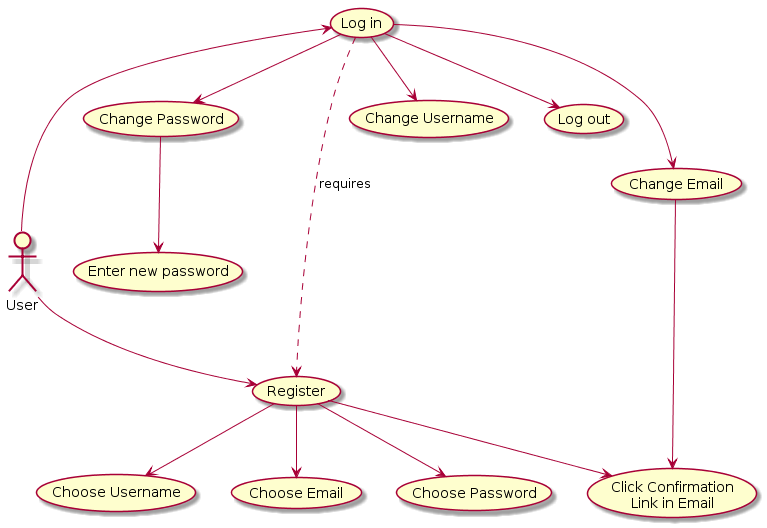
\includegraphics[width=\textwidth]{images/UseCaseDiagrams/Authentication}

\newpage

\subsubsection[Authentication Feature 1: Sign Up Use Case Description]{\selectlanguage{english}\rmfamily\bfseries\color{black}
Authentication Feature 1: Sign Up Use Case Description}
\hypertarget{RefHeading22059017292}{}

\vspace{2pt}
\hrule
\vspace{8pt}
\textbf{Actors:} User \newline

\noindent\textbf{Summary:} The user signs up and creates an account using their email address and creates username and password in order to access the program. \newline

\noindent\textbf{Purpose:} To register and create an account in the program \newline

\noindent\textbf{Preconditions:} None \newline

\noindent\textbf{Steps:} \begin{enumerate}
	\item User clicks Register button.
	\item System prompts the user to enter email and password.
	\item User enters email and password and clicks Submit button.
	\item System sends confirmation email.
	\item User verifies email by clicking a link.
	\item System adds verified user to database.
\end{enumerate}
\noindent\textbf{Alternative 1:} User already has an account. \newline

\noindent\textbf{Alternative 2:} User doesn't confirm email. Delete request after timeout period. \newline

\noindent\textbf{Relevant Classes:}
\begin{itemize}
	\item \textbf{User} in \textbf{S3.4.5}
	\item \textbf{Email} in \textbf{S3.4.5}
	\item \textbf{Validator} in \textbf{S3.4.5}
	\item \textbf{UserController} to be added.
	\item \textbf{ServerController} to be added.
	\item \textbf{Database} to be added.
\end{itemize}
\vspace{8pt}
\hrule
\newpage

\subsubsection[Authentication Feature 1: Sign Up Sequence Diagram]{\selectlanguage{english}\rmfamily\bfseries\color{black}
	Authentication Feature 1: Sign Up Sequence Diagram}
\hypertarget{RefHeading22059017292}{}

\bigskip

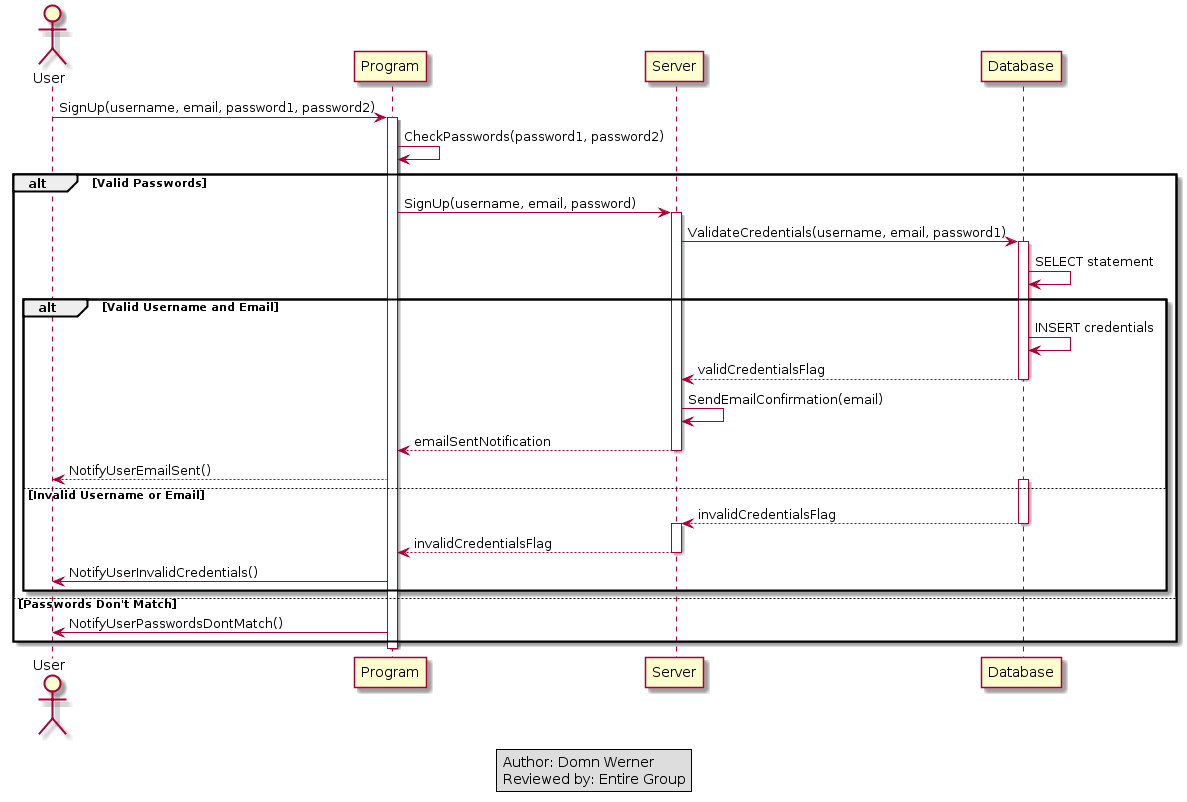
\includegraphics[width=\textwidth]{images/SequenceDiagrams/AuthenticationSignUp}

\newpage

\subsubsection[Authentication Feature 2: Log In Use Case Description]{\selectlanguage{english}\rmfamily\bfseries\color{black}
	Authentication Feature 2: Log In Use Case Description}
\hypertarget{RefHeading22059017292}{}

\hrule
\vspace{8pt}
\noindent\textbf{Actors:} User \newline

\noindent\textbf{Summary:} A registered logs in to the program in order to access its features.  \newline

\noindent\textbf{Purpose:} Allow registered users access to the program.  \newline

\noindent\textbf{Preconditions:} User must already have a registered account.  \newline

\noindent\textbf{Steps:}
\begin{enumerate}
	\item Users clicks Log In button.
	\item System prompts the user for their username and password.
	\item User enters their login information.
	\item System verifies the login information and grants user access to their account.
\end{enumerate}
\noindent\textbf{Alternatives:}
	\begin{enumerate}
		\item User enters incorrect information. System prompts for credentials again.
		\item User has not clicked email confirmation. System resends email and tells user.
		\item User makes 5 incorrect login attempts. System prevents more login attempts for 5 minutes.
	\end{enumerate}

\noindent\textbf{Relevant Classes:}
\begin{itemize}
	\item \textbf{User} in \textbf{S3.4.5}
	\item \textbf{UserController} to be added.
	\item \textbf{ServerController} to be added.
	\item \textbf{Database} to be added.
\end{itemize}
\vspace{8pt}
\hrule
\newpage

\subsubsection[Authentication Feature 2: Log In Sequence Diagram]{\selectlanguage{english}\rmfamily\bfseries\color{black}
	Authentication Feature 2: Log In Sequence Diagram}
\hypertarget{RefHeading22059017292}{}

\bigskip

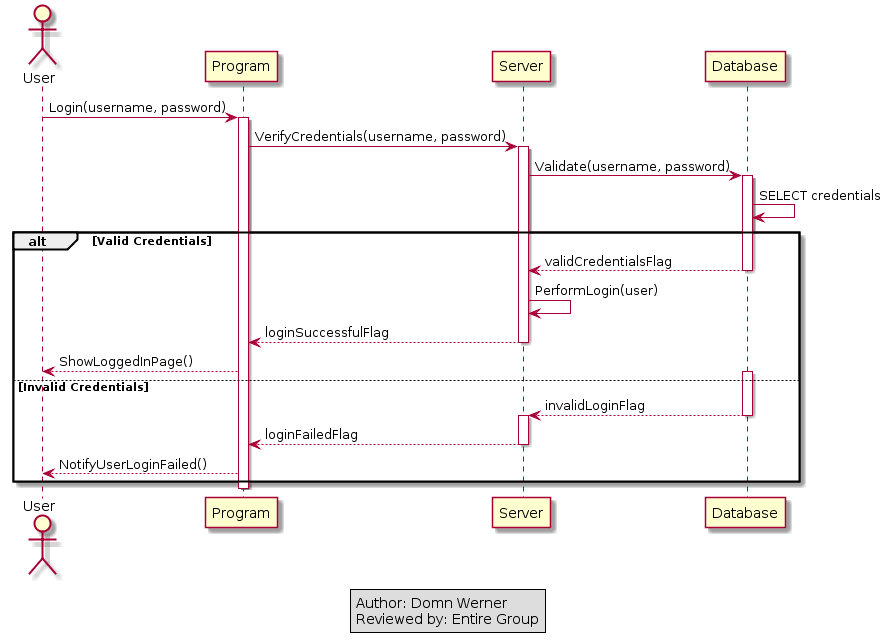
\includegraphics[width=\textwidth]{images/SequenceDiagrams/AuthenticationLogIn}

\newpage

\subsubsection[Authentication Feature 3: Log Out Use Case Description]{\selectlanguage{english}\rmfamily\bfseries\color{black}
	Authentication Feature 3: Log Out Use Case Description}
\hypertarget{RefHeading22059017292}{}

\hrule
\vspace{8pt}
\noindent\textbf{Actors:} User \newline

\noindent\textbf{Summary:} A user logs out of the program.  \newline

\noindent\textbf{Purpose:} Allows logged in users to log out in order to protect their account.  \newline

\noindent\textbf{Preconditions:}
\begin{enumerate}
	\item User must have a registered account.
	\item User must be logged in.
\end{enumerate}

\noindent\textbf{Steps:}
\begin{enumerate}
	\item Users clicks log out button.
	\item System logs user out.
	\item Browser cookies are updated to reflect user being logged out.
\end{enumerate}

\noindent\textbf{Relevant Classes:}
\begin{itemize}
	\item \textbf{User} in \textbf{S3.4.5}
	\item \textbf{UserController} to be added.
	\item \textbf{ServerController} to be added.
	\item \textbf{Database} to be added.
\end{itemize}
\vspace{8pt}
\hrule
\newpage

\subsubsection[Authentication Feature 3: Log Out Sequence Diagram]{\selectlanguage{english}\rmfamily\bfseries\color{black}
	Authentication Feature 3: Log Out Sequence Diagram}
\hypertarget{RefHeading22059017292}{}

\bigskip

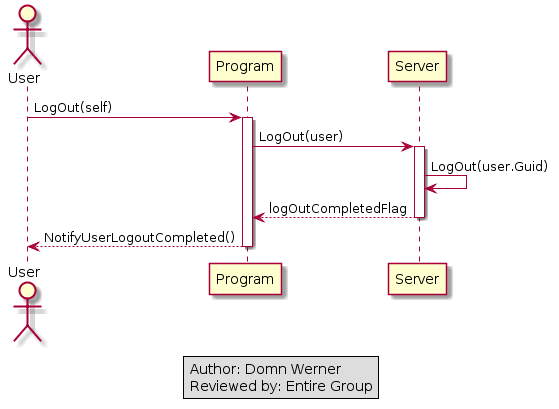
\includegraphics[width=\textwidth]{images/SequenceDiagrams/AuthenticationLogOut}

\newpage

\subsubsection[Authentication Feature 4: Change Password Use Case Description]{\selectlanguage{english}\rmfamily\bfseries\color{black}
	Authentication Feature 4: Change Password Use Case Description}
\hypertarget{RefHeading22059017292}{}

\hrule
\vspace{8pt}
\noindent\textbf{Actors:} User \newline

\noindent\textbf{Summary:} A user changes their password while logged in.  \newline

\noindent\textbf{Purpose:} Allows logged in users to change their passwords.  \newline

\noindent\textbf{Preconditions:}
\begin{enumerate}
	\item User must have a registered account.
	\item User must be logged in.
\end{enumerate}

\noindent\textbf{Steps:}
\begin{enumerate}
	\item Users clicks Change Password button.
	\item System prompts user to enter their password twice.
	\item User enters their password twice.
	\item System hashes both passwords.
\end{enumerate}

\noindent\textbf{Alternatives:}
\begin{enumerate}
	\item If passwords match, System updates user password and sends email to registered email account.
	\item If passwords don't match, system notifies user.
\end{enumerate}

\noindent\textbf{Related Use Cases:}
\begin{enumerate}
	\item Change Email
	\item Change Username
\end{enumerate}

\noindent\textbf{Relevant Classes:}
\begin{itemize}
	\item \textbf{User} in \textbf{S3.4.5}.
	\item \textbf{Email} in \textbf{S3.4.5}.
	\item \textbf{Validator} in \textbf{S3.4.5}.
	\item \textbf{UserController} to be added.
	\item \textbf{ServerController} to be added.
	\item \textbf{Database} to be added.
\end{itemize}
\vspace{8pt}
\hrule
\newpage

\subsubsection[Authentication Feature 4: Change Password Sequence Diagram]{\selectlanguage{english}\rmfamily\bfseries\color{black}
	Authentication Feature 4: Change Password Sequence Diagram}
\hypertarget{RefHeading22059017292}{}

\bigskip

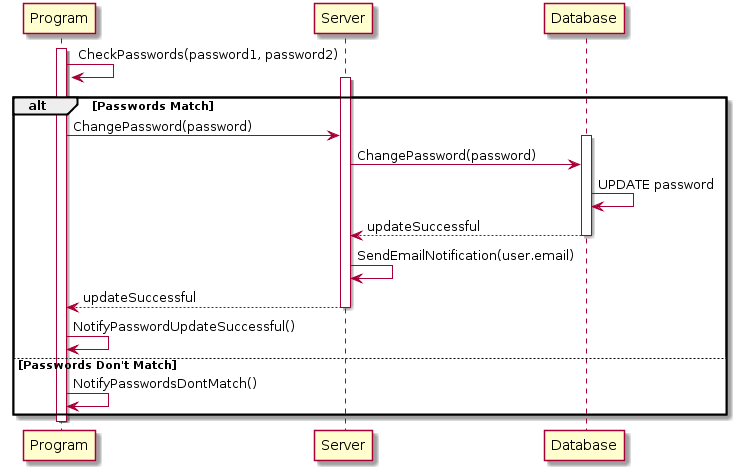
\includegraphics[width=\textwidth]{images/SequenceDiagrams/AuthenticationChangePassword}

\newpage

\subsubsection[Authentication Feature 5: Change Email Use Case Description]{\selectlanguage{english}\rmfamily\bfseries\color{black}
	Authentication Feature 5: Change Email Use Case Description}
\hypertarget{RefHeading22059017292}{}

\hrule
\vspace{8pt}
\noindent\textbf{Actors:} User \newline

\noindent\textbf{Summary:} A user changes their email while logged in.  \newline

\noindent\textbf{Purpose:} Allows logged in users to change their email.  \newline

\noindent\textbf{Preconditions:}
\begin{enumerate}
	\item User must have a registered account.
	\item User must be logged in.
\end{enumerate}

\noindent\textbf{Steps:}
\begin{enumerate}
	\item User clicks Change Email button.
	\item System prompts user to enter their email.
	\item User enters their email.
	\item System sends a confirmation link to the email entered.
\end{enumerate}

\noindent\textbf{Alternatives:}
\begin{enumerate}
	\item If User clicks confirmation link, System updates the user's email and sends an email to the new email stating so.
	\item If user doesn't click confirmation link in an hour, the link becomes invalid.
\end{enumerate}

\noindent\textbf{Related Use Cases:}
\begin{enumerate}
	\item Change Password
	\item Change Username
\end{enumerate}

\noindent\textbf{Relevant Classes:}
\begin{itemize}
	\item \textbf{User} in \textbf{S3.4.5}.
	\item \textbf{Email} in \textbf{S3.4.5}.
	\item \textbf{Validator} in \textbf{S3.4.5}.
	\item \textbf{UserController} to be added.
	\item \textbf{ServerController} to be added.
	\item \textbf{Database} to be added.
\end{itemize}
\vspace{8pt}
\hrule
\newpage

\subsubsection[Authentication Feature 5: Change Email Sequence Diagram]{\selectlanguage{english}\rmfamily\bfseries\color{black}
	Authentication Feature 5: Change Email Sequence Diagram}
\hypertarget{RefHeading22059017292}{}

\bigskip

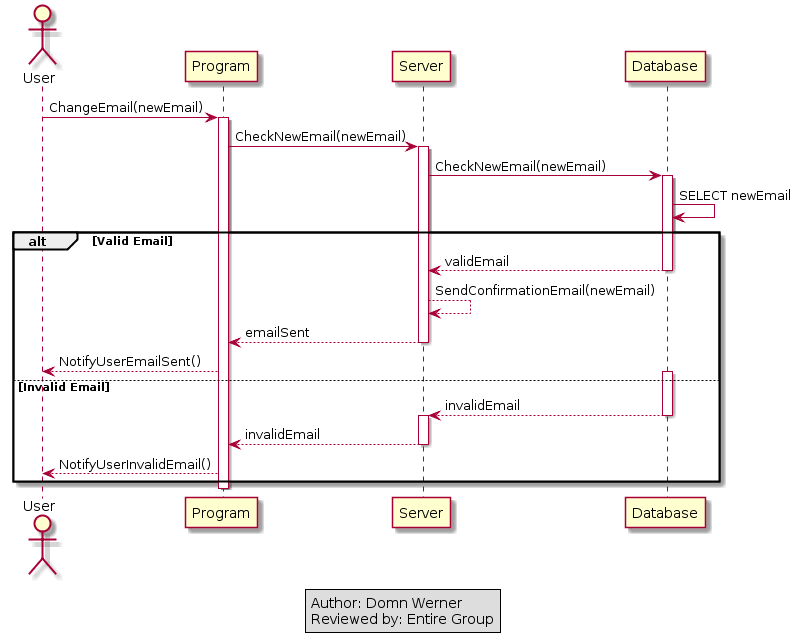
\includegraphics[width=\textwidth]{images/SequenceDiagrams/AuthenticationChangeEmail}

\newpage

\subsubsection[Authentication Feature 6: Change Username Use Case Description] {\selectlanguage{english}\rmfamily\bfseries\color{black}
	Authentication Feature 6: Change Username Use Case Description}
\hypertarget{RefHeading22059017292}{}

\hrule
\vspace{8pt}
\noindent\textbf{Actors:} User \newline

\noindent\textbf{Summary:} A user changes their username while logged in.  \newline

\noindent\textbf{Purpose:} Allows logged in users to change their username.  \newline

\noindent\textbf{Preconditions:}
\begin{enumerate}
	\item User must have a registered account.
	\item User must be logged in.
\end{enumerate}

\noindent\textbf{Steps:}
\begin{enumerate}
	\item Users clicks Change Username button.
	\item System prompts user to enter a new username.
	\item User enters a username and clicks Change Username.
\end{enumerate}

\noindent\textbf{Alternatives:}
\begin{enumerate}
	\item If username doesn't exist, System changes the user's username and notifies the user in the UI and through an email.
	\item If username exists, System asks user to enter a different username.
\end{enumerate}

\noindent\textbf{Related Use Cases:}
\begin{enumerate}
	\item Change Password
	\item Change Email
\end{enumerate}

\noindent\textbf{Relevant Classes:}
\begin{itemize}
	\item \textbf{User} in \textbf{S3.4.5}.
	\item \textbf{Email} in \textbf{S3.4.5}.
	\item \textbf{UserController} to be added.
	\item \textbf{ServerController} to be added.
	\item \textbf{Database} to be added.
\end{itemize}
\vspace{8pt}
\hrule
\newpage

\subsubsection[Authentication Feature 6: Change Username Sequence Diagram]{\selectlanguage{english}\rmfamily\bfseries\color{black}
	Authentication Feature 6: Change Username Sequence Diagram}
\hypertarget{RefHeading22059017292}{}

\bigskip

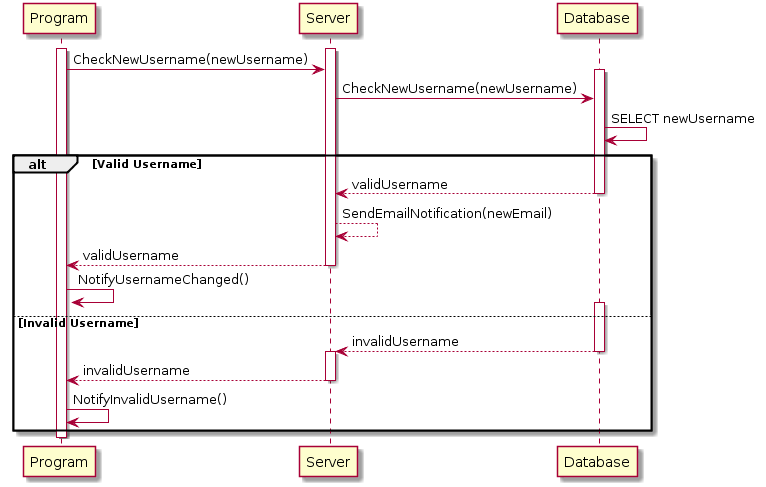
\includegraphics[width=\textwidth]{images/SequenceDiagrams/AuthenticationChangeUsername}

\newpage

\subsubsection[Use Case Diagram 2: Project Browsing]{\selectlanguage{english}\rmfamily\bfseries\color{black}
Use Case Diagram 2: Project Browsing}

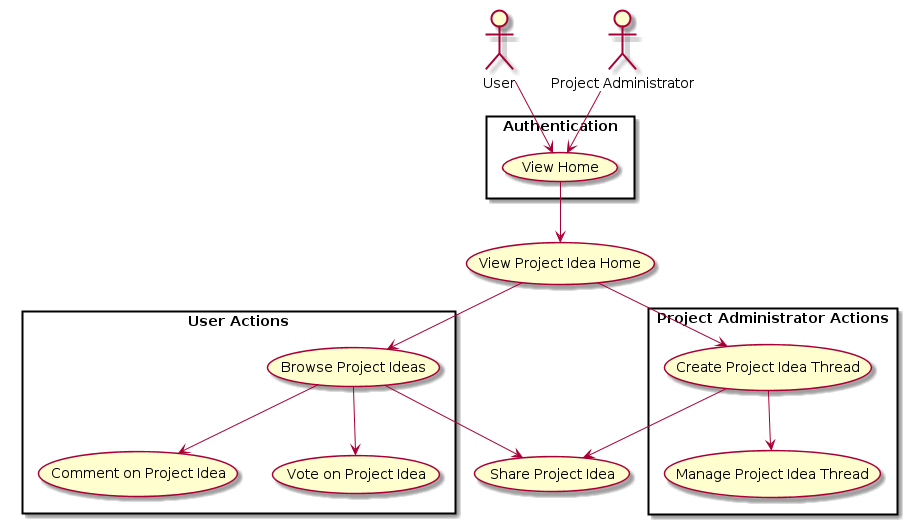
\includegraphics[width=\textwidth]{images/UseCaseDiagrams/ProjectBrowsing}

\newpage

\subsubsection[Project Browsing Feature 1: Project Browsing Use Case Description]{\selectlanguage{english}\rmfamily\bfseries\color{black}
Project Browsing Feature 1: Project Browsing Use Case Description}
\hypertarget{RefHeading22059017292}{}

\vspace{2pt}
\hrule
\vspace{8pt}
\textbf{Actors:} User \newline

\noindent\textbf{Summary:} User looks through posted project ideas to find projects to work on and/or discuss. \newline

\noindent\textbf{Purpose:} To find and view projects relevant to the user's search parameters \newline

\noindent\textbf{Preconditions:} User is signed in \newline

\noindent\textbf{Steps:} \begin{enumerate}
	\item Actor selects Browse Project Ideas button
	\item Actor refines search by selecting from list of project categories as desired
	\item Actor enters terms into search field as desired and views a list of top projects
	\item Actor selects desired project
	\item System displays detailed project information
\end{enumerate}
\noindent\textbf{Alternative 1:} None \newline


\noindent\textbf{Relevant Classes:}
\begin{itemize}
	\item \textbf{User} in \textbf{S3.4.5}
	\item \textbf{Project Browser} in \textbf{S3.4.5}
	\item \textbf{Project} in \textbf{S3.4.5}
\end{itemize}
\vspace{8pt}
\hrule
\newpage
\subsubsection[Project Browsing Feature 1: Project Browsing Sequence Diagram]{\selectlanguage{english}\rmfamily\bfseries\color{black}
	Project Browsing Feature 1: Project Browsing Sequence Diagram}
\hypertarget{RefHeading22059017292}{}

\bigskip

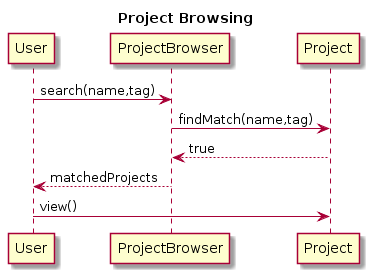
\includegraphics[width=\textwidth]{images/SequenceDiagrams/ProjectBrowsingProjectBrowsing}

\newpage
\subsubsection[Project Browsing Feature 2: Project Creation Use Case Description]{\selectlanguage{english}\rmfamily\bfseries\color{black}
Project Browsing Feature 2: Project Creation Use Case Description}
\hypertarget{RefHeading22059017292}{}

\vspace{2pt}
\hrule
\vspace{8pt}
\textbf{Actors:} User \newline

\noindent\textbf{Summary:} User will create a project. \newline

\noindent\textbf{Purpose:} To allow users to create projects and make them accessible to other users \newline

\noindent\textbf{Preconditions:} User is signed in \newline

\noindent\textbf{Steps:} \begin{enumerate}
	\item User selects Create Project button
	\item User will enter the information on the project, including its name, goals, and identifying tags.
	\item If project name does not match any existing project, the system will create a project with the specified parameters and set user as an admin for the project.
\end{enumerate}
\noindent\textbf{Alternative 1:} Project name matches the name of an existing project and will ask the user to rename it. \newline


\noindent\textbf{Relevant Classes:}
\begin{itemize}
	\item \textbf{User} in \textbf{S3.4.5}
	\item \textbf{Project Browser} in \textbf{S3.4.5}
	\item \textbf{Project} in \textbf{S3.4.5}
\end{itemize}
\vspace{8pt}
\hrule
\newpage
\subsubsection[Project Browsing Feature 2: Project Creation Sequence Diagram]{\selectlanguage{english}\rmfamily\bfseries\color{black}
	Project Browsing Feature 2: Project Creation Sequence Diagram}
\hypertarget{RefHeading22059017292}{}

\bigskip

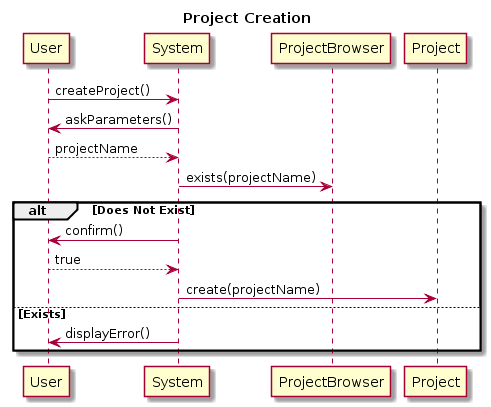
\includegraphics[width=\textwidth]{images/SequenceDiagrams/ProjectBrowsingProjectCreation}

\newpage
\subsubsection[Project Browsing Feature 3: Project Commenting Use Case Description]{\selectlanguage{english}\rmfamily\bfseries\color{black}
Project Browsing Feature 3: Project Commenting Use Case Description}
\hypertarget{RefHeading22059017292}{}

\vspace{2pt}
\hrule
\vspace{8pt}
\textbf{Actors:} User \newline

\noindent\textbf{Summary:} Provide detailed feedback on project ideas  \newline

\noindent\textbf{Purpose:} To allow users to write longform feedback on projects as necessary. \newline

\noindent\textbf{Preconditions:} User is signed in \newline

\noindent\textbf{Steps:} \begin{enumerate}
	\item User selects Comment button
	\item User types feedback into field
	\item User clicks Submit button
	\item System shows confirmation that feedback was received
\end{enumerate}
\noindent\textbf{Alternative 1:} If the project requires comments to be made by project members only and the user is not a project member, the user will be shown an error message. \newline


\noindent\textbf{Relevant Classes:}
\begin{itemize}
	\item \textbf{User} in \textbf{S3.4.5}
	\item \textbf{Project} in \textbf{S3.4.5}
\end{itemize}
\vspace{8pt}
\hrule
\newpage
\subsubsection[Project Browsing Feature 3: Project Commenting Sequence Diagram]{\selectlanguage{english}\rmfamily\bfseries\color{black}
	Project Browsing Feature 3: Project Commenting Sequence Diagram}
\hypertarget{RefHeading22059017292}{}

\bigskip

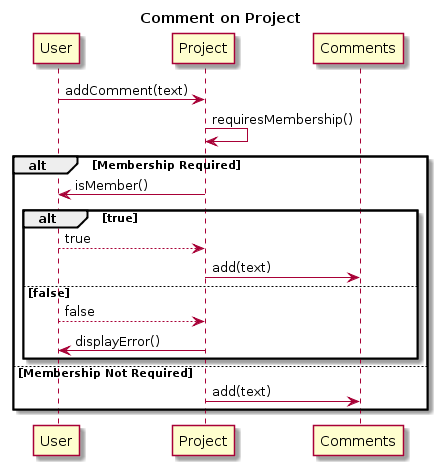
\includegraphics[width=\textwidth]{images/SequenceDiagrams/ProjectBrowsingProjectCommenting}

\newpage
\subsubsection[Project Browsing Feature 4: Project Voting Use Case Description]{\selectlanguage{english}\rmfamily\bfseries\color{black}
Project Browsing Feature 4: Project Voting Use Case Description}
\hypertarget{RefHeading22059017292}{}

\vspace{2pt}
\hrule
\vspace{8pt}
\textbf{Actors:} User \newline

\noindent\textbf{Summary:} Support promising project ideas or offer criticism to unfavorable ones  \newline

\noindent\textbf{Purpose:} Allow for feedback and help users search for well received projects \newline

\noindent\textbf{Preconditions:} User is signed in \newline

\noindent\textbf{Steps:} \begin{enumerate}
	\item User selects Browse Project Ideas button
	\item User refines search by selecting from list of project categories as desired
	\item User enters terms into search field as desired and views a list of top projects
	\item User selects desired project
	\item System displays detailed project information
	\item User selects Up Vote or Down Vote button
	\item Project receives the vote and updates its total score
\end{enumerate}
\noindent\textbf{Alternative 1:} None \newline


\noindent\textbf{Relevant Classes:}
\begin{itemize}
	\item \textbf{User} in \textbf{S3.4.5}
	\item \textbf{Project Browser} in \textbf{S3.4.5}
	\item \textbf{Project} in \textbf{S3.4.5}
\end{itemize}
\hrule
\newpage
\subsubsection[Project Browsing Feature 4: Project Voting Sequence Diagram]{\selectlanguage{english}\rmfamily\bfseries\color{black}
	Project Browsing Feature 4: Project Voting Sequence Diagram}
\hypertarget{RefHeading22059017292}{}

\bigskip

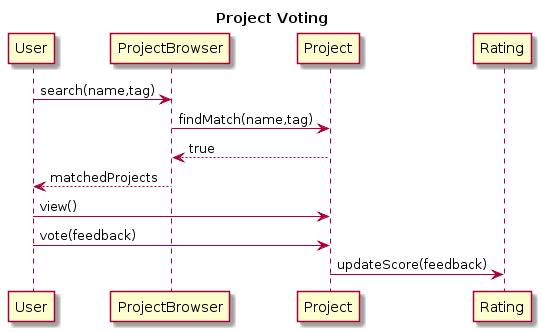
\includegraphics[width=\textwidth]{images/SequenceDiagrams/ProjectBrowsingProjectVoting}

\newpage

\subsubsection[Use Case Diagram 3: Communication]{\selectlanguage{english}\rmfamily\bfseries\color{black}
	Use Case Diagram 3: Communication}

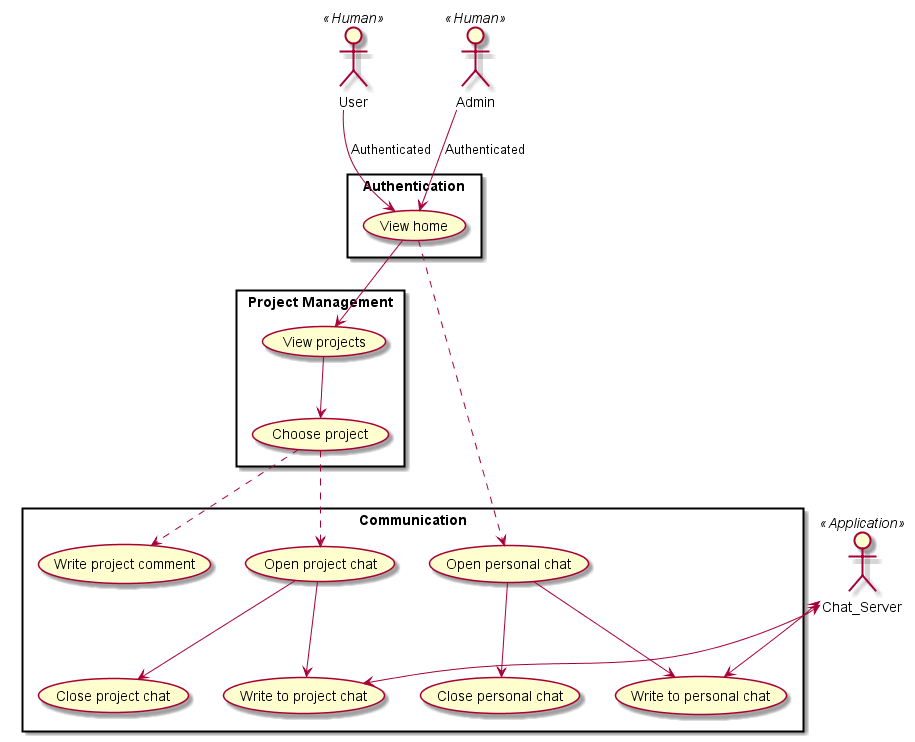
\includegraphics[width=\textwidth]{images/UseCaseDiagrams/Communication}

\newpage

\subsubsection[Communication Feature 1: Read Project Chat Use Case Description]{\selectlanguage{english}\rmfamily\bfseries\color{black}
	Communication Feature 1: Read Project Chat Use Case Description}
\hypertarget{RefHeading22059017292}{}

\vspace{2pt}
\hrule
\vspace{8pt}
\textbf{Actors:} User \newline

\noindent\textbf{Summary:} Open a window to view the conversation in a project  \newline

\noindent\textbf{Purpose:} Allow users to communicate quickly without permanently taking up screen space in a project \newline

\noindent\textbf{Preconditions:} User is signed in and viewing a project \newline

\noindent\textbf{Steps:} \begin{enumerate}
	\item User selects the "Open Chat" button
	\item System opens the chat window, and notifies the other users in the project of the new arrival
	\item System displays any messages from other users in the project in that window until it is closed/left.
\end{enumerate}
\noindent\textbf{Alternative 1:} None \newline


\noindent\textbf{Relevant Classes:}
\begin{itemize}
	\item \textbf{User}
	\item \textbf{TextChat}
	\item \textbf{ChatDisplay}
	\item \textbf{Message}
\end{itemize}
\hrule
\newpage

\subsubsection[Communication Feature 1: Read Project Chat Sequence Diagram]{\selectlanguage{english}\rmfamily\bfseries\color{black}
	Communication Feature 1: Read Project Chat Sequence Diagram}
\hypertarget{RefHeading22059017292}{}

\bigskip

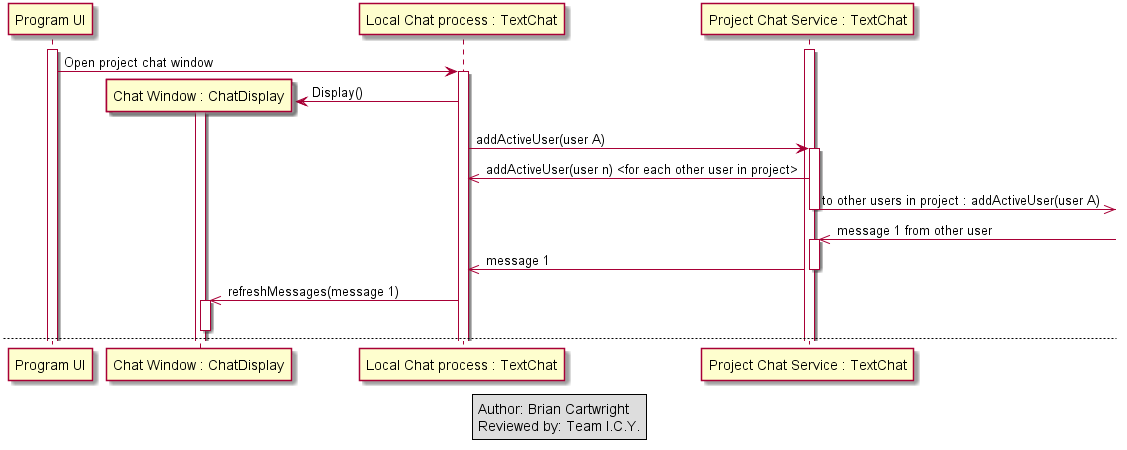
\includegraphics[width=\textwidth]{images/SequenceDiagrams/Comms_OpenRead}

\newpage

\subsubsection[Communication Feature 2: Write to Project Chat Use Case Description]{\selectlanguage{english}\rmfamily\bfseries\color{black}
	Communication Feature 2: Write to Project Chat Use Case Description}
\hypertarget{RefHeading22059017292}{}

\vspace{2pt}
\hrule
\vspace{8pt}
\textbf{Actors:} at least one User \newline

\noindent\textbf{Summary:} Contribute to the conversation in a project  \newline

\noindent\textbf{Purpose:} Allow users to communicate quickly without permanently taking up screen space in a project \newline

\noindent\textbf{Preconditions:} User is signed in and has joined the project chat \newline

\noindent\textbf{Steps:} \begin{enumerate}
	\item User types a message in the project chat window and presses Send
	\item System sends that message to the project server, which delivers it to the other users in the project chat
	\item Other users may read and/or respond to the message at their leisure
\end{enumerate}
\noindent\textbf{Alternative 1:} None \newline


\noindent\textbf{Relevant Classes:}
\begin{itemize}
	\item \textbf{User}
	\item \textbf{TextChat}
	\item \textbf{ChatDisplay}
	\item \textbf{Message}
\end{itemize}
\hrule
\newpage

\subsubsection[Communication Feature 2: Write to Project Chat Sequence Diagram]{\selectlanguage{english}\rmfamily\bfseries\color{black}
	Feature 2: Write to Project Chat Sequence Diagram}
\hypertarget{RefHeading22059017292}{}

\bigskip

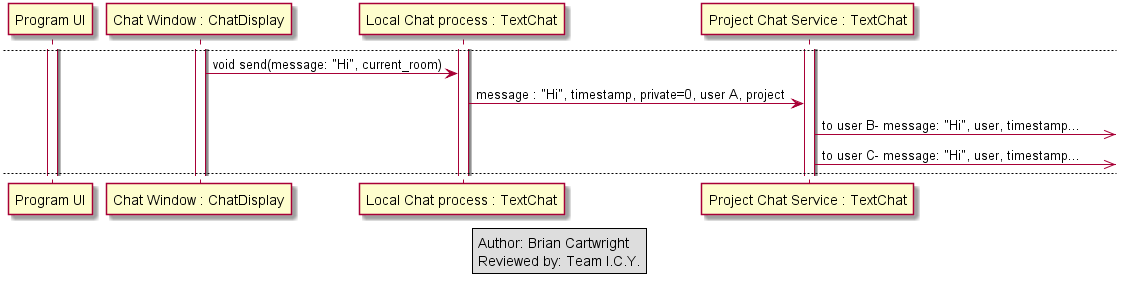
\includegraphics[width=\textwidth]{images/SequenceDiagrams/Comms_WriteToProject}

\newpage

\subsubsection[Communication Feature 3: Message User by Name Use Case Description]{\selectlanguage{english}\rmfamily\bfseries\color{black}
	Communication Feature 3: Message User by Name Use Case Description}
\hypertarget{RefHeading22059017292}{}

\vspace{2pt}
\hrule
\vspace{8pt}
\textbf{Actors:} User \newline

\noindent\textbf{Summary:} Start talking an individual user \newline

\noindent\textbf{Purpose:} Allow users to communicate outside of a project, or in private \newline

\noindent\textbf{Preconditions:} At least one of the users are signed in \newline

\noindent\textbf{Steps:} \begin{enumerate}
	\item User selects "Send PM" from the chat menu and types or selects the other user's ID
	\item System checks to see if the user exists and is online, and if so creates a chat channel for the two users
	\item Both users then use the chat as normal
\end{enumerate}
\noindent\textbf{Alternative 1:} If the second user exists but is offline, the first user is notified and the second user gets the message from the server the next time they're online. \newline


\noindent\textbf{Relevant Classes:}
\begin{itemize}
	\item \textbf{User}
	\item \textbf{TextChat}
	\item \textbf{ChatDisplay}
	\item \textbf{Message}
\end{itemize}
\hrule
\newpage

\subsubsection[Communication Feature 3: Message User by Name Sequence Diagram]{\selectlanguage{english}\rmfamily\bfseries\color{black}
	Feature 3: Message User by Name Sequence Diagram}
\hypertarget{RefHeading22059017292}{}

\bigskip

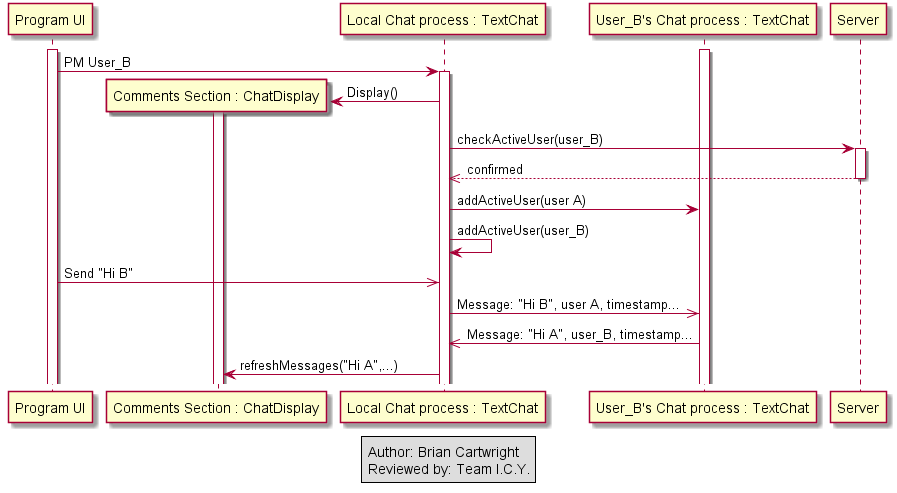
\includegraphics[width=\textwidth]{images/SequenceDiagrams/Comms_PM}

\newpage

\subsubsection[Communication Feature 4: Comment on Project Use Case Description]{\selectlanguage{english}\rmfamily\bfseries\color{black}
	Communication Feature 4: Comment on Project Use Case Description}
\hypertarget{RefHeading22059017292}{}

\vspace{2pt}
\hrule
\vspace{8pt}
\textbf{Actors:} User, sometimes also a Project Admin \newline

\noindent\textbf{Summary:} Communicate more important info about a project  \newline

\noindent\textbf{Purpose:} Allow users to record and semi-permanently attach messages to be displayed alongside a project \newline

\noindent\textbf{Preconditions:} User is signed in and has joined the project \newline

\noindent\textbf{Steps:} \begin{enumerate}
	\item In a section of the window seperate from temporary chat, the user writes a comment and presses Post
	\item System sends that message to the project server, which attaches it to the project. The message is then displayed with previous comments in the post.
	\item Other users may read and/or respond to the message at their leisure
\end{enumerate}
\noindent\textbf{Alternative 1:} A project administrator may remove the post. \newline


\noindent\textbf{Relevant Classes:}
\begin{itemize}
	\item \textbf{User}
	\item \textbf{TextChat}
	\item \textbf{ChatDisplay}
	\item \textbf{Message}
\end{itemize}
\hrule
\newpage

\subsubsection[Communication Feature 4: Comment on Project Sequence Diagram]{\selectlanguage{english}\rmfamily\bfseries\color{black}
	Feature 4: Comment on Project Sequence Diagram}
\hypertarget{RefHeading22059017292}{}

\bigskip

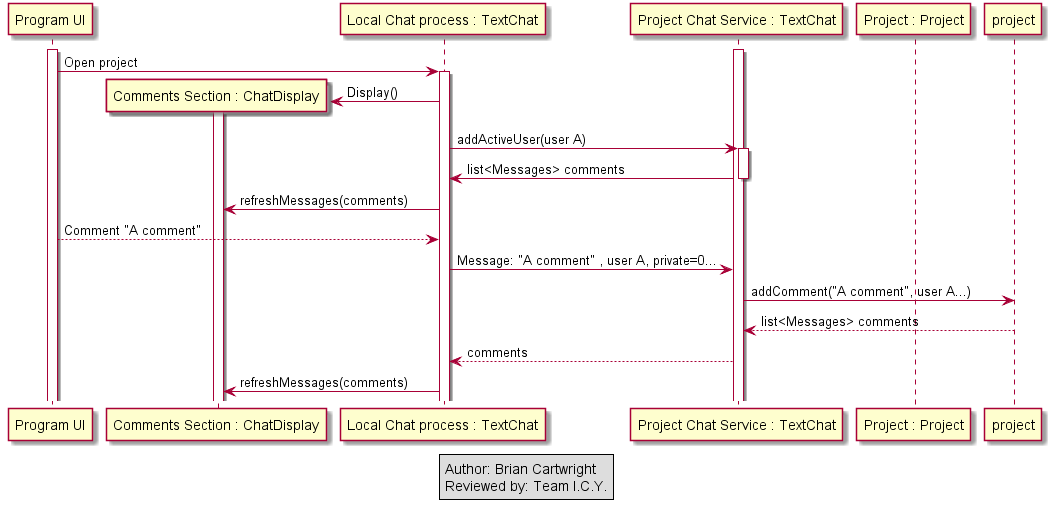
\includegraphics[width=\textwidth]{images/SequenceDiagrams/Comms_LeaveComment}

\newpage

\subsubsection[Communication Feature 5: Close chat Use Case Description]{\selectlanguage{english}\rmfamily\bfseries\color{black}
	Communication Feature 4: Comment on Project Use Case Description}
\hypertarget{RefHeading22059017292}{}

\vspace{2pt}
\hrule
\vspace{8pt}
\textbf{Actors:} User or Admin \newline

\noindent\textbf{Summary:} Clean up when a user leaves a project chat \newline

\noindent\textbf{Purpose:} Close the window and remove the user from the list of active users in the project chat so they don't receive more messages \newline

\noindent\textbf{Preconditions:} User is signed in and has joined the project chat \newline

\noindent\textbf{Steps:} \begin{enumerate}
	\item User clicks "close" on the project chat window
	\item System minimizes the window, and removes the user from the list of active users in the project chat
\end{enumerate}
\noindent\textbf{Alternatives: Step one is skipped if one of the following happen: }
\begin{enumerate}
	\item The user closes the entire project or program windows
	\item The user is idle for too long
	\item An administrator removes them from the project or project chat
\end{enumerate}


\noindent\textbf{Relevant Classes:}
\begin{itemize}
	\item \textbf{User}
	\item \textbf{TextChat}
	\item \textbf{ChatDisplay}
	\item \textbf{Message}
\end{itemize}
\hrule
\newpage

\subsubsection[Communication Feature 5: Close chat Sequence Diagram]{\selectlanguage{english}\rmfamily\bfseries\color{black}
	Feature 5: Close chat Sequence Diagram}
\hypertarget{RefHeading22059017292}{}

\bigskip

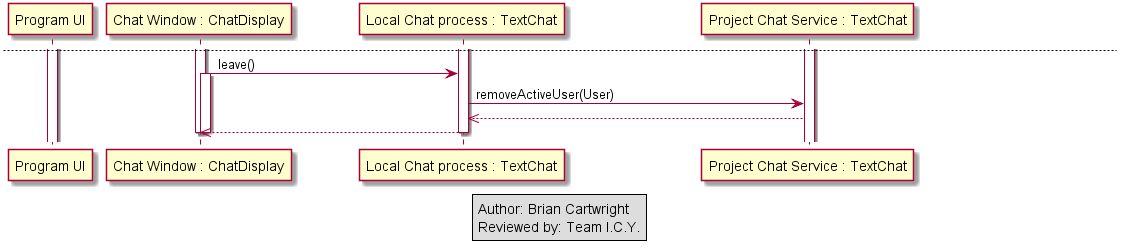
\includegraphics[width=\textwidth]{images/SequenceDiagrams/Comms_CloseProjectChat}

\newpage


\subsubsection[Project Browsing Feature 2: Use Case Description 2]{\selectlanguage{english}\rmfamily\bfseries\color{black}
	Project Browsing Feature 2: Use Case Description 2}
\hypertarget{RefHeading22059017292}{}
\bigskip

{\selectlanguage{english}\color{black}
	\foreignlanguage{english}{\textit{For each feature, you should either provide a Use Case Description
		}}\foreignlanguage{english}{\textbf{\textit{or}}}\foreignlanguage{english}{\textit{ a Non-task feature description,
		whichever is more appropriate.}}}
\newpage

\subsubsection[Use Case Diagram 4: User Preferences]{\selectlanguage{english}\rmfamily\bfseries\color{black}
	Use Case Diagram 4: User Preferences}

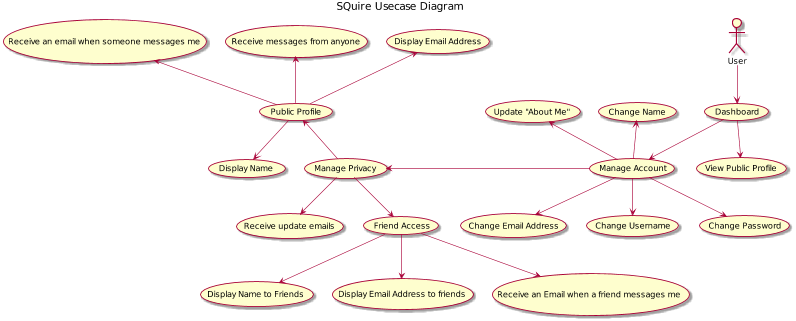
\includegraphics[width=\textwidth]{images/UseCaseDiagrams/UserPreferences}

\newpage

\subsubsection[User Preferences Feature 1: Use Case Description 1]{\selectlanguage{english}\rmfamily\bfseries\color{black}
	User Preferences Feature 1: Use Case Description 1}
\hypertarget{RefHeading22059017292}{}
\bigskip

{\selectlanguage{english}\color{black}
	\foreignlanguage{english}{\textit{For each feature, you should either provide a Use Case Description
		}}\foreignlanguage{english}{\textbf{\textit{or}}}\foreignlanguage{english}{\textit{ a Non-task feature description,
		whichever is more appropriate.}}}
\newpage

\subsubsection[User Preferences Feature 2: Use Case Description 2]{\selectlanguage{english}\rmfamily\bfseries\color{black}
	User Preferences Feature 2: Use Case Description 2}
\hypertarget{RefHeading22059017292}{}
\bigskip

{\selectlanguage{english}\color{black}
	\foreignlanguage{english}{\textit{For each feature, you should either provide a Use Case Description
		}}\foreignlanguage{english}{\textbf{\textit{or}}}\foreignlanguage{english}{\textit{ a Non-task feature description,
		whichever is more appropriate.}}}
\newpage

\subsubsection[Use Case Diagram 5: Project Management (dani2918)]{\selectlanguage{english}\rmfamily\bfseries\color{black}
	Use Case Diagram 5: Project Management}
Use case descriptions were roughly based upon cases from HW2, Team 4. sass8427 worked on the original use cases in this section.


\newpage



\subsubsection[Project Management Feature 1: Use Case Description 1: Compile and execute project (dani2918)]{\selectlanguage{english}\rmfamily\bfseries\color{black}
	Project Management Feature 1: Compile and execute project (dani2918) }
\hypertarget{RefHeading22059017292}{}
\bigskip
\vspace{2pt}
\hrule
\vspace{8pt}
 \textbf{Actors:} User \newline
 
\noindent \textbf{Goals:} Compile and execute active project\newline

 \noindent \textbf{Pre-conditions:} Actor is logged in, navigated to desired project.  \newline
 
\noindent \textbf{Summary:} User compiles a project and the project executes.\newline

\noindent \textbf{Related use cases:} \newline

\noindent \textbf{Steps:} \begin{enumerate}
  \item User clicks ``Compile''
  \item System displays results of compilation
  \item System executes compiled project.
 \end{enumerate}
 \noindent \textbf{Alternatives:} Compilation fails. \newline
 
\noindent  \textbf{Post-conditions:} None. \newline
 
\vspace{8pt}
\hrule

\vspace{20pt}
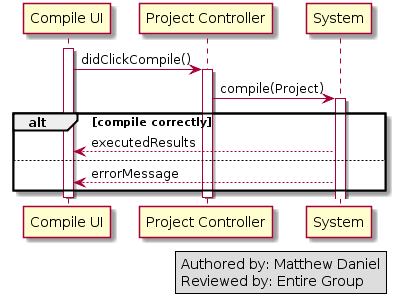
\includegraphics[width=10cm]{images/SequenceDiagrams/PMCompile}

\newpage


\newpage

\subsubsection[Project Management Feature 2: Create project (dani2918)]{\selectlanguage{english}\rmfamily\bfseries\color{black}
	Project Management Feature 2: Create project (dani2918)}
\hypertarget{RefHeading22059017292}{}
\bigskip

\vspace{2pt}
\hrule
\vspace{8pt}
 \noindent \textbf{Actors:} User \newline
 
 \noindent \textbf{Goals:} Create a new project. \newline
 
 \noindent  \textbf{Pre-conditions:} Actor is logged in.  \newline
 
 \noindent \textbf{Summary:} User creates a new project with a description and includes any desired files. \newline
 
 \noindent \textbf{Related use cases:} Import file \newline
 
 \noindent \textbf{Steps:} \begin{enumerate}
  \item User clicks ``New Project.''
  \item User gives project a title.
  \item User adds an applicable description.
  \item User imports any files by clicking ''Import.''
  \item User clicks ``Create''.
  \item System imports files and instantiates project.
 \end{enumerate}
 \textbf{Alternatives:} None. \newline
 
 \noindent  \textbf{Post-conditions:} None. \newline
\vspace{8pt}
\hrule

\vspace{20pt}
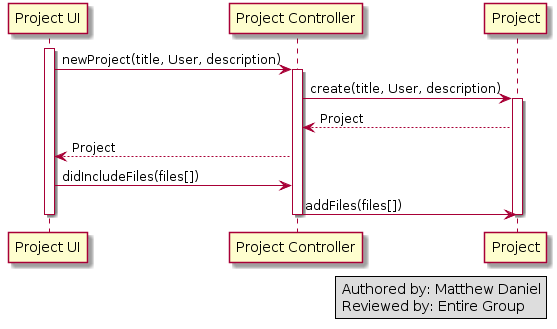
\includegraphics[width=10cm]{images/SequenceDiagrams/PMCreateProject}

\newpage


\subsubsection[Project Management Feature 3: Delete project (dani2918)]{\selectlanguage{english}\rmfamily\bfseries\color{black}
	Project Management Feature 3: Delete project (dani2918)}
\hypertarget{RefHeading22059017292}{}
\bigskip

\vspace{2pt}
\hrule
\vspace{8pt}
 \noindent \textbf{Actors:} Project Administrator, sQuire Administrator. \newline
 
 \noindent \textbf{Goals:} Remove project from sQuire sever. \newline

 \noindent  \textbf{Pre-conditions:} Actor is logged in, viewing desired project.  \newline
 
 \noindent \textbf{Summary:} Actor chooses to delete or remove an irrelevant or inappropriate project.  \newline
 
 \noindent \textbf{Related use cases:} Create project\newline
\textbf{Steps:} \begin{enumerate}
  \item Actor clicks ``Delete'' icon on active project.
  \item Delete dialog opens.
  \item Actor presses ``Delete''.
  \item Confirmation window is displayed.
  \item Actor confirms or disregards deletion.
  \item System notifies collaborators that project was deleted.
 \end{enumerate}
 \textbf{Alternatives:} Actor clicks ``Cancel.'' \newline
 
 \noindent  \textbf{Post-conditions:} None. \newline
\vspace{8pt}
\hrule


\vspace{20pt}
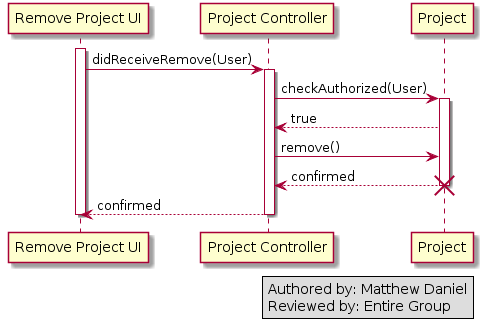
\includegraphics[width=10cm]{images/SequenceDiagrams/PMDeleteProject}


\newpage



\subsubsection[Project Management Feature 4: Request to join project (dani2918)]{\selectlanguage{english}\rmfamily\bfseries\color{black}
	Project Management Feature 4: Request to join project (dani2918)}
\hypertarget{RefHeading22059017292}{}
\bigskip

\vspace{2pt}
\hrule
\vspace{8pt}
\noindent \textbf{Actors:} User \newline

\noindent\textbf{Goals:} Join an existing project. \newline

\noindent \textbf{Pre-conditions:} Actor is logged in, viewing desired project.  \newline

\noindent \textbf{Summary:} Actor sends a request to join as a collaborator on a project\newline

\noindent \textbf{Related use cases:} Manage request to join project\newline

\noindent \textbf{Steps:} \begin{enumerate}
  \item Actor clicks ``Join project.''
  \item Notification is sent to project administrator for review.
 \end{enumerate}
\noindent \textbf{Alternatives:} None. \newline
 
\noindent \textbf{Post-conditions:} None. \newline
\vspace{8pt}
\hrule


\newpage



\subsubsection[Project Management Feature 5: Manage request to join project (dani2918)]{\selectlanguage{english}\rmfamily\bfseries\color{black}
	Project Management Feature 5: Manage request to join project (dani2918)}
\hypertarget{RefHeading22059017292}{}
\bigskip

\vspace{2pt}
\hrule
\vspace{8pt}
\noindent \textbf{Actors:} Project Administrator \newline
 
\noindent \textbf{Goals:} Approve . \newline

\noindent \textbf{Pre-conditions:} Actor is logged in, viewing desired project.  \newline

\noindent \textbf{Summary:} Actor approves/rejects a user who has requested to join as a collaborator on a project.\newline

\noindent \textbf{Related use cases:} Request to join project \newline

\noindent \textbf{Steps:} \begin{enumerate}
  \item Actor clicks ``Review join requests.''
  \item Actor reviews information about potential collaborator.
  \item Actor clicks ``Approve User'' to approve a collaborator or ``Reject user'' to reject a collaborator.
  \item System notifies user that they have been approved/rejected.
 \end{enumerate}
 \textbf{Alternatives:} None. \newline
 
 \noindent  \textbf{Post-conditions:} None. \newline
 \noindent
\vspace{8pt}
\hrule

\vspace{20pt}
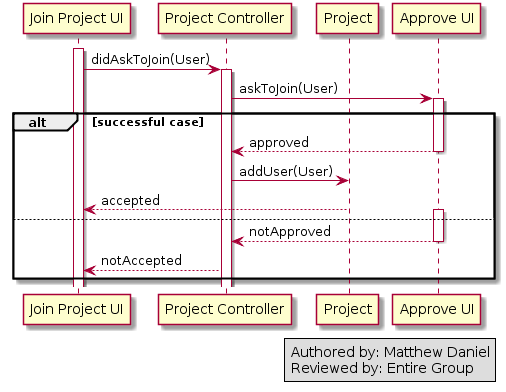
\includegraphics[width=10cm]{images/SequenceDiagrams/PMJoinProject}


\newpage




\subsubsection[Project Management Feature 6: Leave project (dani2918)]{\selectlanguage{english}\rmfamily\bfseries\color{black}
	Project Management Feature 6: Leave project (dani2918)}
\hypertarget{RefHeading22059017292}{}
\bigskip

\vspace{2pt}
\hrule
\vspace{8pt}
\noindent \textbf{Actors:} User \newline

\noindent \textbf{Goals:} Remove actor as a collaborator from project. \newline

\noindent  \textbf{Pre-conditions:} logged in, viewing desired project, collaborator on desired project, not project owner.  \newline

\noindent \textbf{Summary:} A member of a project leaves said project, leaving the project intact. \newline

\noindent \textbf{Related use cases:} Delete project \newline

\noindent \textbf{Steps:} \begin{enumerate}
  \item User clicks ``Leave Project''.
  \item System prompts user to confirm decision.
  \item User clicks "Confirm".
  \item User is removed from project member list.
 \end{enumerate}
 
\noindent  \textbf{Alternatives:} User clicks "Cancel" at step 4. \newline
 
\noindent  \textbf{Post-conditions:} None. \newline
\vspace{8pt}
\hrule
\vspace{20pt}
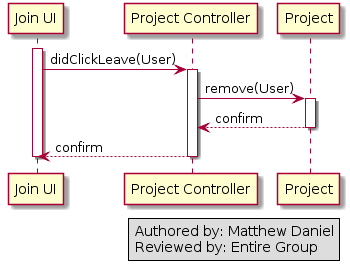
\includegraphics[width=10cm]{images/SequenceDiagrams/PMLeaveProject}

\newpage




\subsubsection[Project Management Feature 7: Invite to project (dani2918)]{\selectlanguage{english}\rmfamily\bfseries\color{black}
	Project Management Feature 7: Invite to project (dani2918)}
\hypertarget{RefHeading22059017292}{}
\bigskip

\vspace{2pt}
\hrule
\vspace{8pt}
\noindent \textbf{Actors:} Project Administrator, Authorized Project Collaborator (User).  \newline

\noindent \textbf{Goals:} Invite user(s) to collaborate on project \newline

\noindent  \textbf{Pre-conditions:} Actor is viewing project which he or she created, is logged in   \newline

\noindent \textbf{Summary:} A project administrator requests help from a user on a project. The sQuire system facilitates the invitation process  \newline

\noindent \textbf{Related use cases:} Respond to project invite\newline

\noindent \textbf{Steps:} \begin{enumerate}
  \item Actor clicks ``Invite User.''
  \item Actor enters the username(s) of the user(s) to be invited to the project.
  \item Actor enters any message to the user(s) in a text box.
  \item Actor clicks ``Send invite.''
  \item System sends notification of invite to user(s).
 \end{enumerate}
 
\noindent  \textbf{Alternatives:} Actor clicks ``Cancel.''
 \textbf{Post-conditions:} None.  \newline
 
\vspace{8pt}
\hrule
\newpage



\subsubsection[Project Management Feature 8: Respond to project invite (dani2918)]{\selectlanguage{english}\rmfamily\bfseries\color{black}
	Project Management Feature 8: Respond to project invite (dani2918)}
\hypertarget{RefHeading22059017292}{}
\bigskip

\vspace{2pt}
\hrule
\vspace{8pt}
\noindent \textbf{Actors:} User  \newline

\noindent \textbf{Goals:} Actor responds to an invitation to a project.\newline

\noindent  \textbf{Pre-conditions:} Actor is signed in, viewing invitation.  \newline

\noindent \textbf{Summary:} Actor receives notification that he or she has been invited to a project and either accepts the invitation or declines it. \newline

\noindent \textbf{Related use cases:} Invite to project \newline

\noindent \textbf{Steps:} \begin{enumerate}
  \item Actor clicks ``Respond to Invitation.''
  \item Actor clicks ``Accept'' or ``Reject.''
  \item Actor types any message to invitation-sender in text box.
  \item Actor clicks ``Confirm.''
 \end{enumerate}
 
\noindent  \textbf{Alternatives:} Actor clicks ``Cancel.'' \newline

\noindent  \textbf{Post-conditions:} Actor becomes collaborator on project if invitation was accepted. \newline
\vspace{8pt}
\hrule
\vspace{20pt}


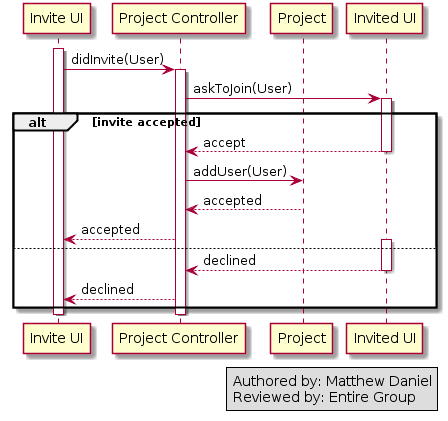
\includegraphics[width=10cm]{images/SequenceDiagrams/PMInviteToProject}
\newpage












\subsubsection[Use Case Diagram 6: File Editing]{\selectlanguage{english}\rmfamily\bfseries\color{black}
	Use Case Diagram 6: File Editing}

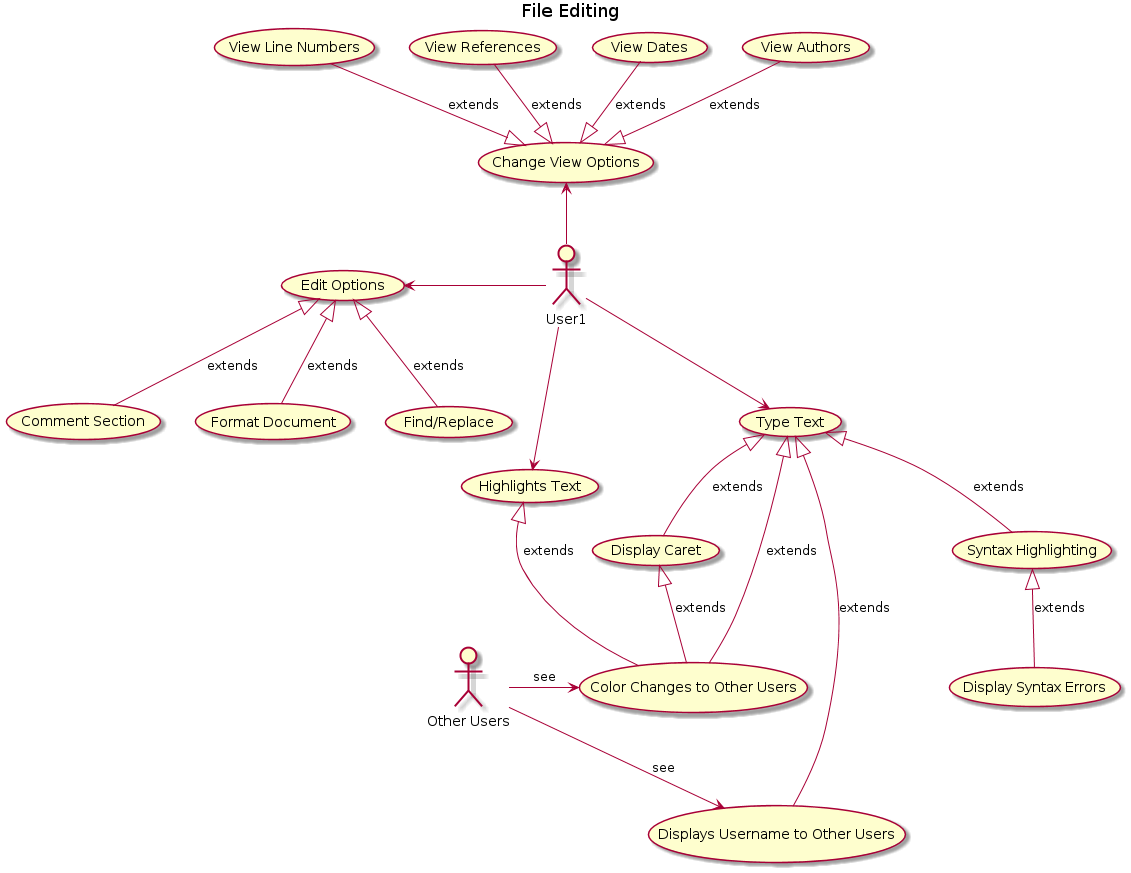
\includegraphics[width=\textwidth]{images/UseCaseDiagrams/FileEditing}

\newpage

\subsubsection[File Editing Feature 1: View Line Numbers]{\selectlanguage{english}\rmfamily\bfseries\color{black}
	File Editing Feature 1: View Line Numbers Use Case Description}
\hypertarget{RefHeading22059017292}{}

\vspace{2pt}
\hrule
\vspace{8pt}
	\noindent\textbf{Name:} View Line Numbers \newline
	\noindent\textbf{Category:} File Editing \newline
	\noindent\textbf{Actor:} User \newline
	\noindent\textbf{Summary:} Allows the user to view line numbers to the left of the document. \newline
	\noindent\textbf{Purpose:} Makes it easier to communicate position in code. It is also a useful metric to have.\newline
	\noindent\textbf{Preconditions:}
	\begin{enumerate}
		\item Must be registered.
		\item Must be logged in.
		\item User has view permission.
		\item A file is open.
	\end{enumerate}
	\noindent\textbf{Steps:}
	\begin{enumerate}
		\item User selects the \textit{View} menu option.
		\item System displays a drop-down with various options.
		\item User selects the \textit{View Line Numbers} option.
		\item System displays line numbers to the left of the document.
	\end{enumerate}
	\noindent\textbf{Relevant Classes:}
	\begin{enumerate}
		\item \textbf {TextOperation}

	\end{enumerate}
\vspace{8pt}
\hrule
\newpage

\subsubsection[File Editing Feature 1: View Line Numbers Sequence Diagram]{\selectlanguage{english}\rmfamily\bfseries\color{black}
	File Editing Feature 1: View Line Numbers Sequence Diagram}
\hypertarget{RefHeading22059017292}{}

\bigskip

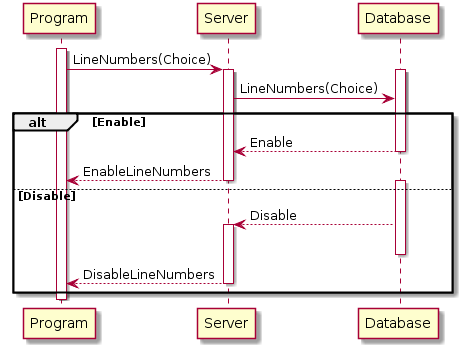
\includegraphics[width=\textwidth]{images/SequenceDiagrams/LineNumbers}

\newpage

\subsubsection[File Editing Feature 2: View References]{\selectlanguage{english}\rmfamily\bfseries\color{black}
	File Editing Feature 2: View References Use Case Description}
\hypertarget{RefHeading22059017292}{}

\vspace{2pt}
\hrule
\vspace{8pt}
	\noindent\textbf{Name:} View References \newline
	\noindent\textbf{Category:} File Editing \newline
	\noindent\textbf{Actor:} User \newline
	\noindent\textbf{Summary:} Allows the user to view the number of references to a given function. \newline
	\noindent\textbf{Purpose:} It is useful to know the number of references to a given function for optimization and debugging purposes. \newline
	\noindent\textbf{Preconditions:}
	\begin{enumerate}
		\item Must be registered.
		\item Must be logged in.
		\item User has view permission.
		\item A \textbf{code} file is open.
	\end{enumerate}
	\noindent\textbf{Steps:}
	\begin{enumerate}
		\item User selects the \textit{View} menu option.
		\item System displays a drop-down with various options.
		\item User selects the \textit{View References} option.
		\item System displays the number of references above each method declaration.
	\end{enumerate}
	\noindent\textbf{Relevant Classes:}
	\begin{enumerate}
		\item \textbf {ColabFile}
		\item \textbf {LineHistory}
		\item \textbf {Project}
	\end{enumerate}
\vspace{8pt}
\hrule
\newpage

\subsubsection[File Editing Feature 2: View References Sequence Diagram]{\selectlanguage{english}\rmfamily\bfseries\color{black}
	File Editing Feature 2: View References Sequence Diagram}
\hypertarget{RefHeading22059017292}{}

\bigskip

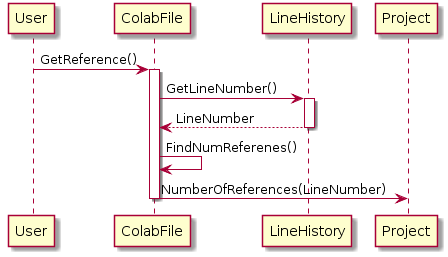
\includegraphics[width=\textwidth]{images/SequenceDiagrams/References}

\newpage

\subsubsection[File Editing Feature 3: View Dates]{\selectlanguage{english}\rmfamily\bfseries\color{black}
	File Editing Feature 3: View Dates Use Case Description}
\hypertarget{RefHeading22059017292}{}

\vspace{2pt}
\hrule
\vspace{8pt}
	\noindent\textbf{Name:} View Dates \newline
	\noindent\textbf{Category:} File Editing \newline
	\noindent\textbf{Actor:} User \newline
	\noindent\textbf{Summary:} Allows the user to view the last date that each line of a document was edited. \newline
	\noindent\textbf{Purpose:} This provides a useful metric for how up-to-date parts of the document are. \newline
	\noindent\textbf{Preconditions:}
	\begin{enumerate}
		\item Must be registered.
		\item Must be logged in.
		\item User has view permission.
		\item A file is open.
	\end{enumerate}
	\noindent\textbf{Steps:}
	\begin{enumerate}
		\item User selects the \textit{View} menu option.
		\item System displays a drop-down with various options.
		\item User selects the \textit{View Dates} option.
		\item System displays the last date that each line of a document was edited.
	\end{enumerate}
	\noindent\textbf{Relevant Classes:}
	\begin{enumerate}
		\item \textbf {LineHistory}
		\item \textbf {FileLineHistory}
	\end{enumerate}
\vspace{8pt}
\hrule
\newpage

\subsubsection[File Editing Feature 3: View Dates Sequence Diagram]{\selectlanguage{english}\rmfamily\bfseries\color{black}
	File Editing Feature 3: View Dates Sequence Diagram}
\hypertarget{RefHeading22059017292}{}

\bigskip

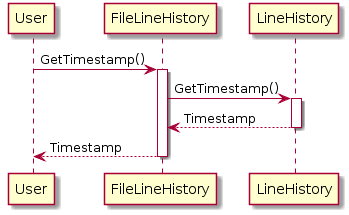
\includegraphics[width=\textwidth]{images/SequenceDiagrams/EditDate}

\newpage

\subsubsection[File Editing Feature 4: View Authors]{\selectlanguage{english}\rmfamily\bfseries\color{black}
	File Editing Feature 4: View Authors Use Case Description}
\hypertarget{RefHeading22059017292}{}

\vspace{2pt}
\hrule
\vspace{8pt}
	\noindent\textbf{Name:} View Authors \newline
	\noindent\textbf{Category:} File Editing \newline
	\noindent\textbf{Actor:} User \newline
	\noindent\textbf{Summary:} Allows the user to view the last author that edited each of line of the document. \newline
	\noindent\textbf{Purpose:} This is an accountability tool allowing other users to identify who is responsible for a change to a document. \newline
	\noindent\textbf{Preconditions:}
	\begin{enumerate}
		\item Must be registered.
		\item Must be logged in.
		\item User has read permission.
		\item A file is open.
	\end{enumerate}
	\noindent\textbf{Steps:}
	\begin{enumerate}
		\item User selects the \textit{View} menu option.
		\item System displays a drop-down with various options.
		\item User selects the \textit{View Authors} option.
		\item System displays the name of the last editor of each line of the document.
	\end{enumerate}
	\noindent\textbf{Relevant Classes:}
	\begin{enumerate}
		\item \textbf {FileLineHistory}
		\item \textbf {LineHistory}
	\end{enumerate}
\vspace{8pt}
\hrule
\newpage

\subsubsection[File Editing Feature 4: View Author Sequence Diagram]{\selectlanguage{english}\rmfamily\bfseries\color{black}
	File Editing Feature 4: View Author Sequence Diagram}
\hypertarget{RefHeading22059017292}{}

\bigskip

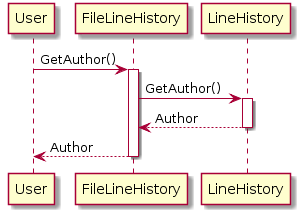
\includegraphics[width=\textwidth]{images/SequenceDiagrams/Author}

\newpage

\subsubsection[File Editing Feature 5: Format Document]{\selectlanguage{english}\rmfamily\bfseries\color{black}
	File Editing Feature 5: Format Document Use Case Description}
\hypertarget{RefHeading22059017292}{}

\vspace{2pt}
\hrule
\vspace{8pt}
	\noindent\textbf{Name:} Format Document \newline
	\noindent\textbf{Category:} File Editing \newline
	\noindent\textbf{Actor:} User \newline
	\noindent\textbf{Summary:} Allows the user to format the document to a specified format \newline
	\noindent\textbf{Purpose:} An easy tool for making sweeping changes to a large part of a document. \newline
	\noindent\textbf{Preconditions:}
	\begin{enumerate}
		\item Must be registered.
		\item Must be logged in.
		\item User has read/write permission.
		\item A file is open.
		\item The document has formatting options set.
	\end{enumerate}
	\noindent\textbf{Steps:}
	\begin{enumerate}
		\item User selects the \textit{Edit} menu option.
		\item System displays a drop-down with various options.
		\item User selects the \textit{Format Document} option.
		\item System formats the current document to the formatting settings currently set.
	\end{enumerate}
	\noindent\textbf{Alternatives:}
	\begin{enumerate}
		\item If no formatting settings are currently set, display a dialog box after step 3 and give the option for the user to do so now.
	\end{enumerate}
	\noindent\textbf{Relevant Classes:}
	\begin{enumerate}
		\item \textbf{TextOperation}
	\end{enumerate}
\vspace{8pt}
\hrule
\newpage

\subsubsection[File Editing Feature 6: Find/Replace]{\selectlanguage{english}\rmfamily\bfseries\color{black}
	File Editing Feature 6: Find/Replace Use Case Description}
\hypertarget{RefHeading22059017292}{}

\vspace{2pt}
\hrule
\vspace{8pt}
	\noindent\textbf{Name:} Find/Replace \newline
	\noindent\textbf{Category:} File Editing \newline
	\noindent\textbf{Actor:} User \newline
	\noindent\textbf{Summary:} Allows the user to find and/or replace phrases. \newline
	\noindent\textbf{Purpose:} This is a powerful tool that allows a user to make safer, quicker, and more efficient changes to a document. \newline
	\noindent\textbf{Preconditions:}
	\begin{enumerate}
		\item Must be registered.
		\item Must be logged in.
		\item User has read/write permission.
		\item A file is open.
	\end{enumerate}
	\noindent\textbf{Steps:}
	\begin{enumerate}
		\item User selects the \textit{Edit} menu option.
		\item System displays a drop-down with various options.
		\item User selects the \textit{Find/Replace} option.
		\item System displays a small form in an unobtrusive location.
		\item User enter the phrase to find and selects find.
		\item System highlights and focuses on the first occurrence of the phrase and all highlights all other occurrences.
	\end{enumerate}
	\noindent\textbf{Alternatives:}
	\begin{enumerate}
		\item User selects option to replace in step 5 and enters a phrase with which to replace the found occurrences of the searched phrase. The system replaces each occurrence.
	\end{enumerate}
	\noindent\textbf{Relevant Classes:}
	\begin{enumerate}
		\item \textbf{Project}
	\end{enumerate}
\hrule
\vspace{8pt}
\newpage

\subsubsection[File Editing Feature 6: Find Sequence Diagram]{\selectlanguage{english}\rmfamily\bfseries\color{black}
	File Editing Feature 6: Find Sequence Diagram}
\hypertarget{RefHeading22059017292}{}

\bigskip

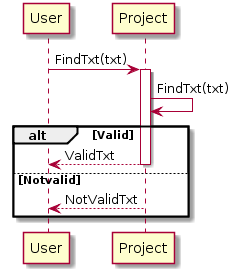
\includegraphics[width=\textwidth]{images/SequenceDiagrams/FindTxt}

\newpage

\subsubsection[File Editing Feature 7: Comment Section]{\selectlanguage{english}\rmfamily\bfseries\color{black}
	File Editing Feature 7: Comment Section Use Case Description}
\hypertarget{RefHeading22059017292}{}

\vspace{2pt}
\hrule
\vspace{8pt}
	\noindent\textbf{Name:} Comment Section \newline
	\noindent\textbf{Category:} File Editing \newline
	\noindent\textbf{Actor:} User \newline
	\noindent\textbf{Summary:} Allows the user to comment out a part of a document. \newline
	\noindent\textbf{Purpose:} A useful and quick way to disable a large part of a document. \newline
	\noindent\textbf{Preconditions:}
	\begin{enumerate}
		\item Must be registered.
		\item Must be logged in.
		\item A file is open.
		\item User has read/write permission.
		\item Current open document supports commenting.
	\end{enumerate}
	\noindent\textbf{Steps:}
	\begin{enumerate}
		\item User selects the \textit{Edit} menu option.
		\item System displays a drop-down with various options.
		\item User selects the \textit{Comment Section} option.
		\item System comments the selected area.
	\end{enumerate}
	\noindent\textbf{Alternatives:}
	\begin{enumerate}
		\item If document does not support commenting, display a dialog box telling the user.
	\end{enumerate}
	\noindent\textbf{Relevant Classes:}
	\begin{enumerate}
		\item \textbf {TextOperation}
	\end{enumerate}
\vspace{8pt}
\hrule
\newpage

\subsubsection[File Editing Feature 7: Comment Section Sequence Diagram]{\selectlanguage{english}\rmfamily\bfseries\color{black}
	File Editing Feature 7: Comment Section Sequence Diagram}
\hypertarget{RefHeading22059017292}{}

\bigskip

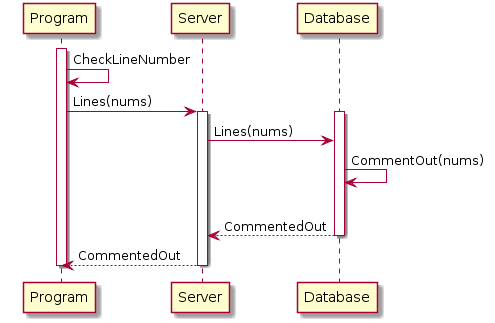
\includegraphics[width=\textwidth]{images/SequenceDiagrams/CommentOut}

\newpage

\subsubsection[File Editing Feature 8: Display Typing User]{\selectlanguage{english}\rmfamily\bfseries\color{black}
	File Editing Feature 8: Display Typing User Use Case Description}
\hypertarget{RefHeading22059017292}{}

\vspace{2pt}
\hrule
\vspace{8pt}
	\noindent\textbf{Name:} Display Typing User \newline
	\noindent\textbf{Category:} File Editing \newline
	\noindent\textbf{Actors:} 
	\begin{enumerate}
		\item User
		\item Other Users
	\end{enumerate}
	\noindent\textbf{Summary:} As the user types, the system displays their name, their typing, and their caret, in a different color, to other users. \newline
	\noindent\textbf{Purpose:} Differentiate who is typing what. \newline
	\noindent\textbf{Preconditions:}
	\begin{enumerate}
		\item Must be registered.
		\item Must be logged in.
		\item User has read/write permission.
		\item A file is open.
		\item Other users have the same document open.
	\end{enumerate}
	\noindent\textbf{Steps:}
	\begin{enumerate}
		\item User begins typing.
		\item System displays the user's typing, the user's name, and the user's caret, in a different color, to Other Users.
		\item Other Users see User typing, his username, and his caret, in a different color.
	\end{enumerate}
	\noindent\textbf{Relevant Classes:}
	\begin{enumerate}
	   \item \textbf {ColabFile}
	   \item \textbf {Cursor}
	   \item \textbf {Project}
	\end{enumerate}
\vspace{8pt}
\hrule
\newpage

\subsubsection[File Editing Feature 8: Display Typing User Sequence Diagram]{\selectlanguage{english}\rmfamily\bfseries\color{black}
	File Editing Feature 8: Display Typing User Sequence Diagram}
\hypertarget{RefHeading22059017292}{}

\bigskip

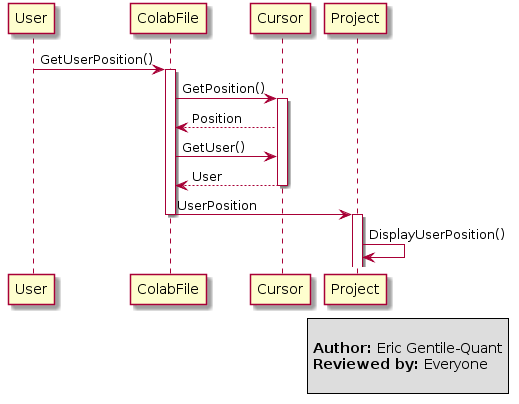
\includegraphics[width=\textwidth]{images/SequenceDiagrams/UserPosition}

\newpage


\subsubsection[File Editing Feature 9: Display Syntax Errors]{\selectlanguage{english}\rmfamily\bfseries\color{black}
	File Editing Feature 9: Display Syntax Errors Use Case Description}
\hypertarget{RefHeading22059017292}{}

\vspace{2pt}
\hrule
\vspace{8pt}
	\noindent\textbf{Name:} Display Syntax Errors \newline
	\noindent\textbf{Category:} File Editing \newline
	\noindent\textbf{Actor:} User \newline
	\noindent\textbf{Summary:} As the user types code, the editor will underline syntax errors with a red line. \newline
	\noindent\textbf{Purpose:} Aids the user is writing correct code. \newline
	\noindent\textbf{Preconditions:}
	\begin{enumerate}
		\item Must be registered.
		\item Must be logged in.
		\item User has read/write permission.
		\item A supported code file is open.
	\end{enumerate}
	\noindent\textbf{Steps:}
	\begin{enumerate}
		\item User begins typing.
		\item System displays any syntax errors as a red underline under the incorrect section.
	\end{enumerate}
	\noindent\textbf{Relevant Classes:}
	\begin{enumerate}
	    \item \textbf {ColabFile}
	    \item \textbf {Project}
	\end{enumerate}    
\vspace{8pt}
\hrule
\newpage

\subsubsection[File Editing Feature 9: Display Syntax Errors Sequence Diagram]{\selectlanguage{english}\rmfamily\bfseries\color{black}
	File Editing Feature 9: Display Syntax Errors Sequence Diagram}
\hypertarget{RefHeading22059017292}{}

\bigskip

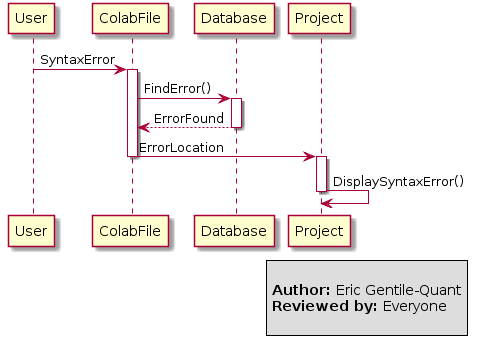
\includegraphics[width=\textwidth]{images/SequenceDiagrams/SyntaxError}

\newpage

\subsubsection[File Editing Feature 10: Display Syntax Highlighting]{\selectlanguage{english}\rmfamily\bfseries\color{black}
	File Editing Feature 10: Display Syntax Highlighting Use Case Description}
\hypertarget{RefHeading22059017292}{}

\vspace{2pt}
\hrule
\vspace{8pt}
	\noindent\textbf{Name:} Display Syntax Highlighting \newline
	\noindent\textbf{Category:} File Editing \newline
	\noindent\textbf{Actor:} User \newline
	\noindent\textbf{Summary:} As the user types code, the editor will change font color for different code structures and keywords. \newline
	\noindent\textbf{Purpose:} Aids the user is writing code and identifying key code parts. \newline
	\noindent\textbf{Preconditions:}
	\begin{enumerate}
		\item Must be registered.
		\item Must be logged in.
		\item User has read/write permission.
		\item A supported code file is open.
	\end{enumerate}
	\noindent\textbf{Steps:}
	\begin{enumerate}
		\item User begins typing.
		\item System automatically colors special code structures and keywords.
	\end{enumerate}
	\noindent\textbf{Relevant Classes:}
	\begin{enumerate}
	    \item \textbf {Project}
	\end{enumerate}
\vspace{8pt}
\hrule
\newpage

\subsubsection[File Editing Feature 10: Display Syntax Highlighting Sequence Diagram]{\selectlanguage{english}\rmfamily\bfseries\color{black}
	File Editing Feature 10: Display Syntax Highlighting Sequence Diagram}
\hypertarget{RefHeading22059017292}{}

\bigskip

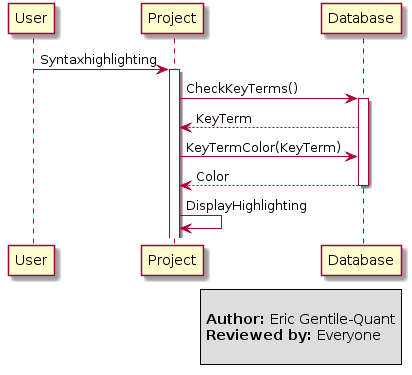
\includegraphics[width=\textwidth]{images/SequenceDiagrams/SyntaxHighlighting}

\newpage


\subsubsection[Use Case Diagram 7: File Management]{\selectlanguage{english}\rmfamily\bfseries\color{black}
	Use Case Diagram 7: File Management}
\hypertarget{RefHeading22059017292}{}

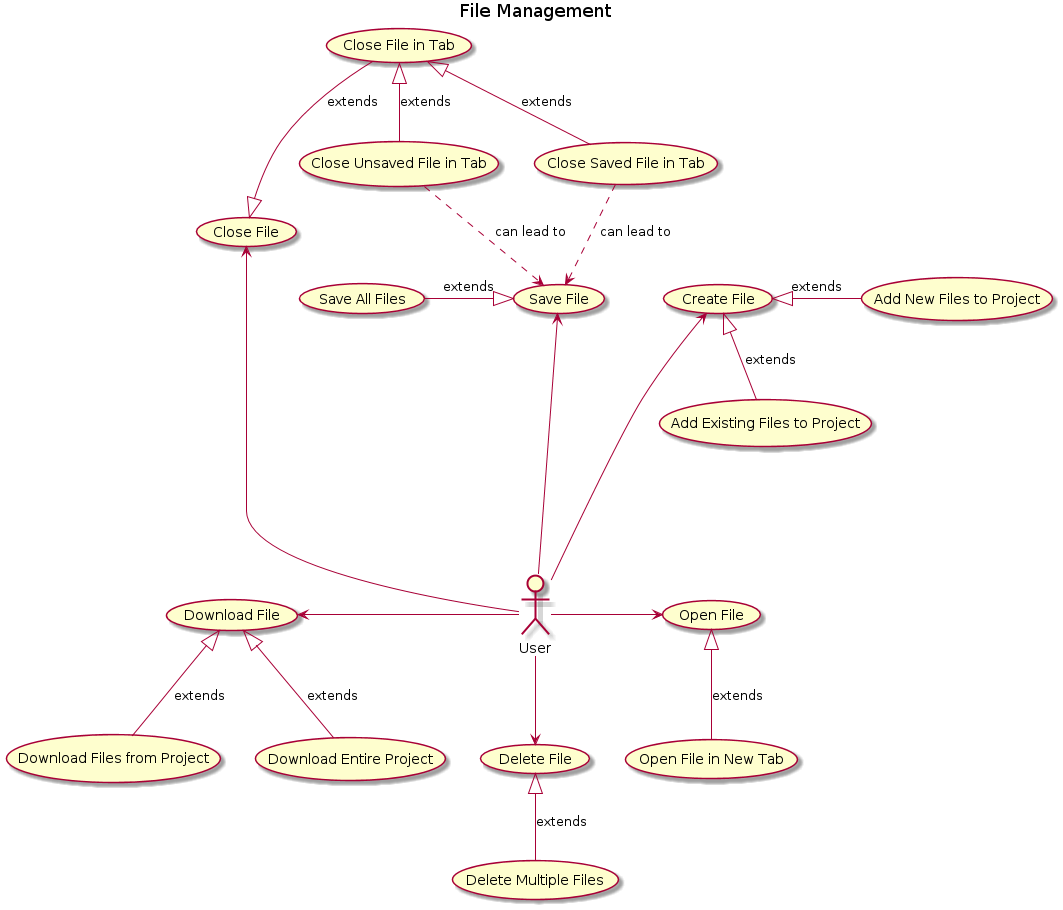
\includegraphics[width=\textwidth]{images/UseCaseDiagrams/FileManagement}

\newpage

\subsubsection[File Management Feature 1: Open File Use Case Description]{\selectlanguage{english}\rmfamily\bfseries\color{black}
	File Management Feature 1: Open File Use Case Description}
\hypertarget{RefHeading22059017292}{}

\vspace{2pt}
\hrule
\vspace{8pt}
\textbf{Actors:} User \newline

\noindent\textbf{Summary:} The user selects a file to open based on a filename, which is then opened by the software. \newline

\noindent\textbf{Purpose:} To open a file in the program. \newline

\noindent\textbf{Preconditions:} The desired file must already exist. \newline

\noindent\textbf{Steps:}
\begin{enumerate}
	\item User clicks Open File button.
	\item System prompts the user to select file to open from a list of existing files.
	\item User selects desired file and clicks Submit button.
	\item System opens selected file and displays it.
\end{enumerate}
\noindent\textbf{Alternative 1:} The User decides they don't want to open a file and presses Cancel at step 3. \newline

\noindent\textbf{Relevant Classes:}
\begin{itemize}
	\item \textbf{User} in \textbf{S3.4.5}
	\item \textbf{UI} to be added.
	\item \textbf{Project} to be added.
	\item \textbf{File} to be added.
\end{itemize}

\hrule

\newpage

\subsubsection[File Management Feature 1: Open File Sequence Diagram]{\selectlanguage{english}\rmfamily\bfseries\color{black}
	File Management Feature 1: Open File Sequence Diagram}
\hypertarget{RefHeading22059017292}{}

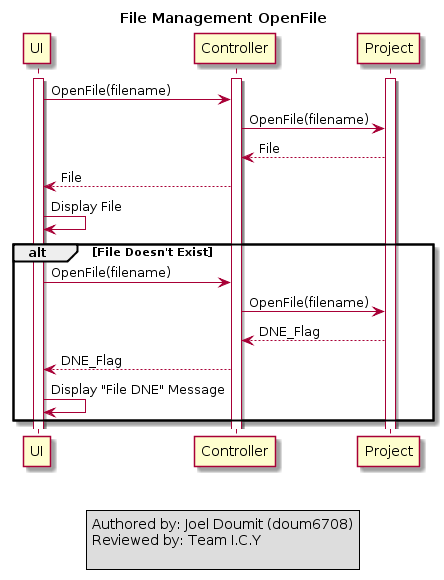
\includegraphics[width=\textwidth]{images/SequenceDiagrams/FM_OpenFile_Image}

\newpage

\subsubsection[File Management Feature 2: Close File Use Case Description]{\selectlanguage{english}\rmfamily\bfseries\color{black}
	File Management Feature 2: Close File Use Case Description}
\hypertarget{RefHeading22059017292}{}

\vspace{2pt}
\hrule
\vspace{8pt}
\textbf{Actors:} User \newline

\noindent\textbf{Summary:} The user chooses to close the file they are working on. \newline

\noindent\textbf{Purpose:} To close a file in the program. \newline

\noindent\textbf{Preconditions:} The desired file must already exist, and be already opened by the User. \newline

\noindent\textbf{Steps:}
\begin{enumerate}
	\item User clicks Close File button.
	\item System closes the file and updates the Controller's status on the file being open.
\end{enumerate}

\noindent\textbf{Alternative 1:} The file cannot be closed for some reason. \newline

\noindent\textbf{Relevant Classes:}
\begin{itemize}
	\item \textbf{User} in \textbf{S3.4.5}
	\item \textbf{UI} to be added.
	\item \textbf{Project} to be added.
	\item \textbf{File} to be added.
\end{itemize}
\vspace{8pt}
\hrule

\newpage

\subsubsection[File Management Feature 2: Close File Sequence Diagram]{\selectlanguage{english}\rmfamily\bfseries\color{black}
	File Management Feature 2: Close File Sequence Diagram}
\hypertarget{RefHeading22059017292}{}

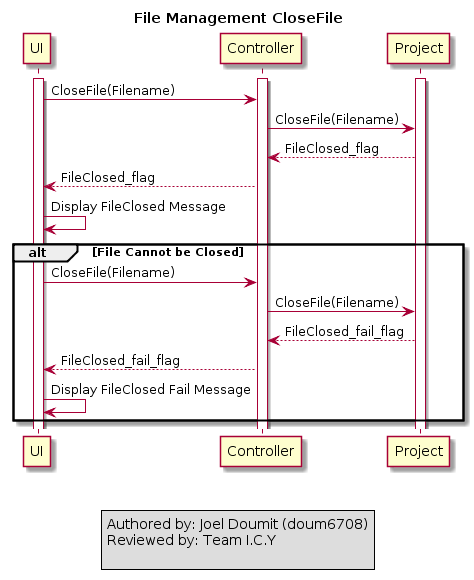
\includegraphics[width=\textwidth]{images/SequenceDiagrams/FM_FileClose_Image}

\newpage

\subsubsection[File Management Feature 3: Save File Use Case Description]{\selectlanguage{english}\rmfamily\bfseries\color{black}
	File Management Feature 3: Save File Use Case Description}
\hypertarget{RefHeading22059017292}{}

\vspace{2pt}
\hrule
\vspace{8pt}
\textbf{Actors:} User \newline

\noindent\textbf{Summary:} The user chooses to save the file they are currently working on. \newline

\noindent\textbf{Purpose:} To save a file in the program. \newline

\noindent\textbf{Preconditions:} The desired file must already exist, and be opened by the user. \newline

\noindent\textbf{Steps:} \begin{enumerate}
	\item User clicks Save File button.
	\item System prompts the user to choose a name to save the file under.
	\item User selects desired name and clicks Submit button.
	\item System saves selected file and allows the user to keep working.

\end{enumerate}
\noindent\textbf{Alternative 1:} The User decides they don't want to save the file and presses Cancel at step 3. \newline

\noindent\textbf{Relevant Classes:}
\begin{itemize}
	\item \textbf{User} in \textbf{S3.4.5}
	\item \textbf{UI} to be added.
	\item \textbf{Project} to be added.
	\item \textbf{File} to be added.
\end{itemize}
\vspace{8pt}
\hrule

\newpage

\subsubsection[File Management Feature 3: Save File Sequence Diagram]{\selectlanguage{english}\rmfamily\bfseries\color{black}
	File Management Feature 3: Save File Sequence Diagram}
\hypertarget{RefHeading22059017292}{}

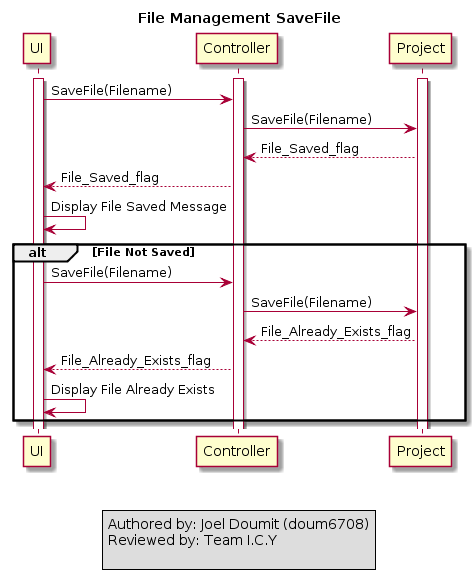
\includegraphics[width=\textwidth]{images/SequenceDiagrams/FM_SaveFile_Image}

\newpage

\subsubsection[File Management Feature 4: Add File Use Case Description]{\selectlanguage{english}\rmfamily\bfseries\color{black}
	File Management Feature 4: Add File Use Case Description}
\hypertarget{RefHeading22059017292}{}

\vspace{2pt}
\hrule
\vspace{8pt}
\textbf{Actors:} User \newline

\noindent\textbf{Summary:} The user chooses to add a file to the directory. \newline

\noindent\textbf{Purpose:} To add a file to a directory. \newline

\noindent\textbf{Preconditions:} The desired file must already exist. \newline

\noindent\textbf{Steps:} \begin{enumerate}
	\item User clicks Add File button.
	\item System prompts the user to choose a file to add to a directory..
	\item User selects desired file and clicks Submit button.
	\item System prompts the user to choose a directory to add the file to.
	\item User selects directory to add the file to and click Submit button.
	\item System adds the file to the selected directory and lets the user return to their work.

\end{enumerate}
\noindent\textbf{Alternative 1:} The User decides they don't want to add the file and presses Cancel at step 3. \newline
\noindent\textbf{Alternative 2:} The User decides, after they chose a file, not to add it to a directory and clicks Cancel at step 5. \newline

\noindent\textbf{Relevant Classes:}
\begin{itemize}
	\item \textbf{User} in \textbf{S3.4.5}
	\item \textbf{UI} to be added.
	\item \textbf{Project} to be added.
	\item \textbf{File} to be added.
\end{itemize}
\vspace{8pt}
\hrule
\bigskip

\newpage

\subsubsection[File Management Feature 4: Add File Sequence Diagram]{\selectlanguage{english}\rmfamily\bfseries\color{black}
	File Management Feature 4: Add File Sequence Diagram}
\hypertarget{RefHeading22059017292}{}

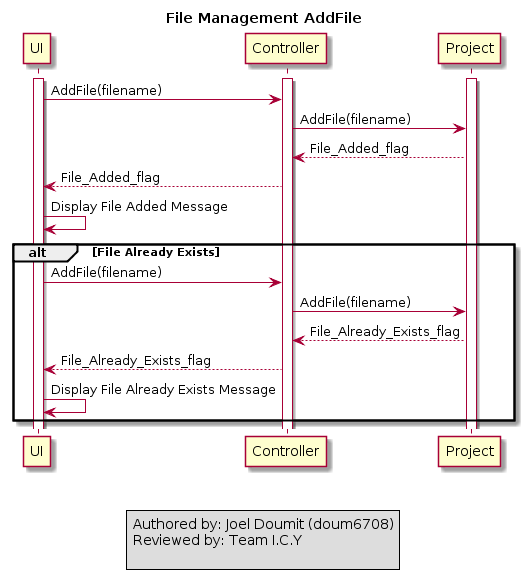
\includegraphics[width=\textwidth]{images/SequenceDiagrams/FM_AddFile_Image}

\newpage

\subsubsection[Use Case Diagram 8: Project User Management]{\selectlanguage{english}\rmfamily\bfseries\color{black}
	Use Case Diagram 8: Project User Management}

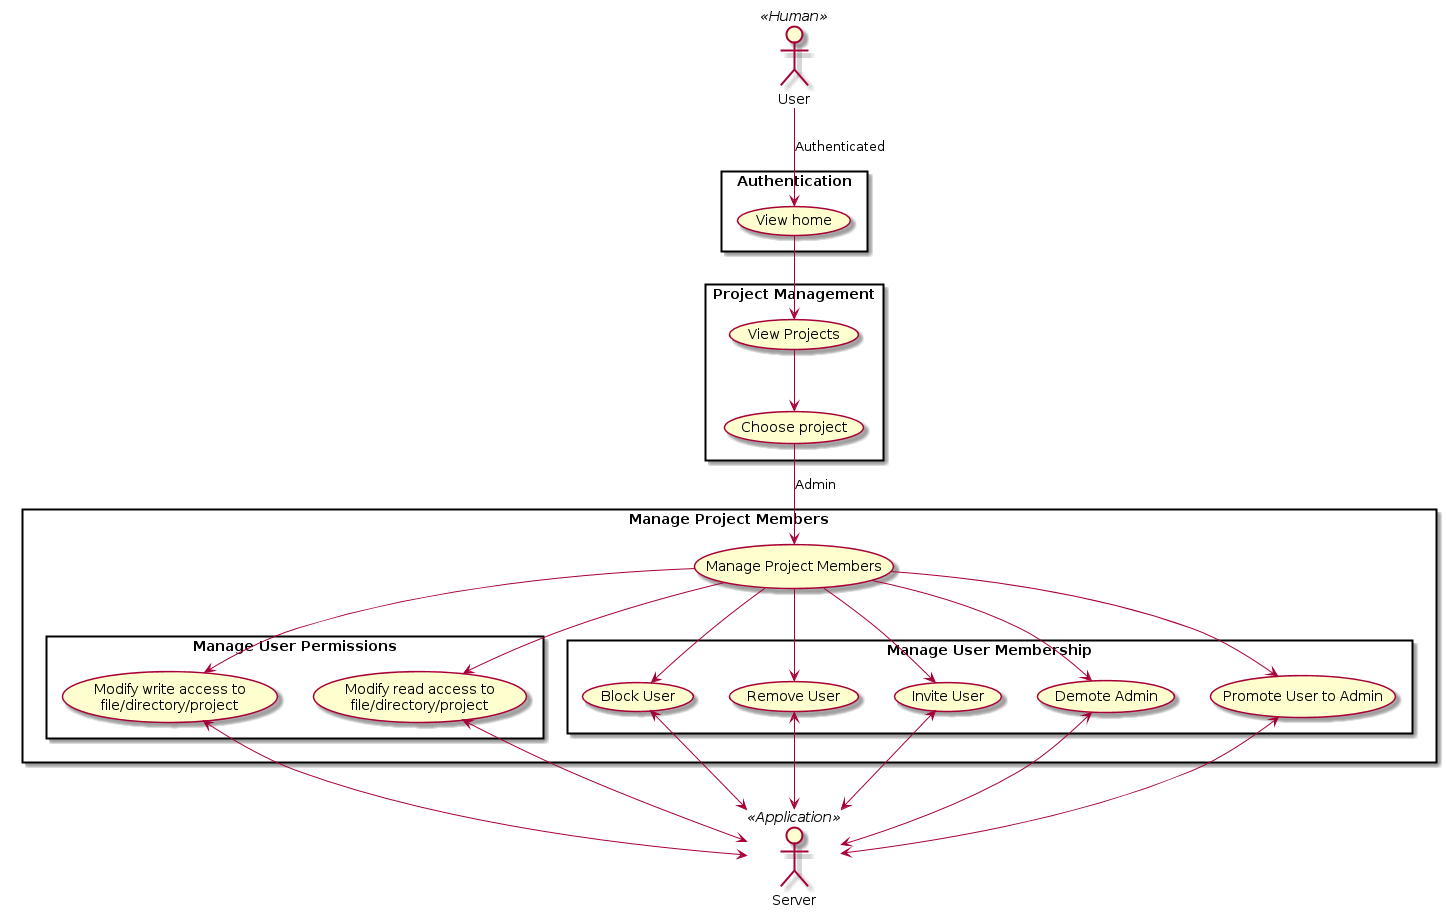
\includegraphics[width=\textwidth]{images/UseCaseDiagrams/ProjectUserManagement}

\newpage

\subsubsection[Project User Management Feature 1: Add User to Project Use Case Description]{\selectlanguage{english}\rmfamily\bfseries\color{black}
	Project User Management Feature 1: Add User to Project Use Case Description}
\hypertarget{RefHeading22059017292}{}

\vspace{2pt}
\hrule
\vspace{8pt}
 \textbf{Actors:} User \newline
\textbf{Goals:} Add a user to project \newline
 \textbf{Pre-conditions:} User has admin rights to project. \newline
 \textbf{Summary:} User adds a user to a project \newline
\textbf{Related use cases:} Kick User \newline
\textbf{Steps:} \begin{enumerate}
  \item User clicks add user button.
  \item System prompts user to enter the username of the user they wish to invite.
  \item User enters username.
  \item System adds the specified user to the project, and notifies them.
 \end{enumerate}
 \textbf{Alternatives:} \begin{enumerate}
  \item User enters an invalid username, in which case an error is reported
 \end{enumerate}
 \textbf{Post-conditions:} None. \newline
\vspace{8pt}
\textbf{Relevant Classes:}
\begin{itemize}
	\item \textbf{User}
	\item \textbf{Project}
	\item \textbf{UserManager}
	\item \textbf{Permissions}
	\item \textbf{Email}
\end{itemize}
\hrule
\newpage

\subsubsection[Project User Management Feature 1: Add User Sequence Diagram]{\selectlanguage{english}\rmfamily\bfseries\color{black}
	Project User Management Feature 1: Add User Sequence Diagram}
\hypertarget{RefHeading22059017292}{}

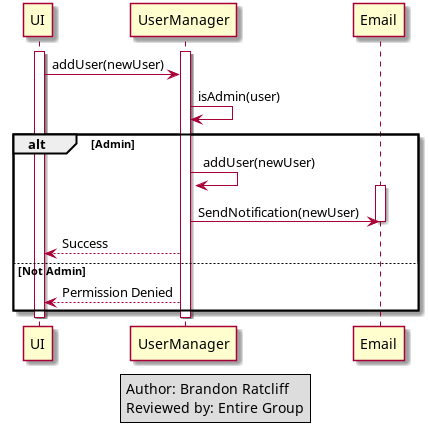
\includegraphics[width=\textwidth]{images/SequenceDiagrams/ProjectUserManagementAddUser}

\newpage
\subsubsection[Project User Management Feature 2: Kick User Use Case Description]{\selectlanguage{english}\rmfamily\bfseries\color{black}
	Project User Management Feature 2: Kick User Use Case Description}
\hypertarget{RefHeading22059017292}{}

\vspace{2pt}
\hrule
\vspace{8pt}
 \textbf{Actors:} User \newline
\textbf{Goals:} Kick a user from project. \newline
 \textbf{Pre-conditions:} User is an admin, and the user they wish to kick is a membor of the project. \newline
 \textbf{Summary:} User removes a selected user from the Project \newline
\textbf{Related use cases:} Add User \newline
\textbf{Steps:} \begin{enumerate}
  \item User clicks Kick User button.
  \item System displays list of Members of the project.
  \item User selects one or more other users from the list and presses Remove.
  \item System prompts User for verification.
  \item User presses Confirm.
  \item System removes the selected users from the project.
 \end{enumerate}
 \textbf{Alternatives:} None. \newline
 \textbf{Post-conditions:} None. \newline
\begin{itemize}
	\item \textbf{User}
	\item \textbf{Project}
	\item \textbf{UserManager}
	\item \textbf{Permissions}
\end{itemize}
\vspace{8pt}
\hrule
\newpage

\subsubsection[Project User Management Feature 2: Kick User Sequence Diagram]{\selectlanguage{english}\rmfamily\bfseries\color{black}
	Project User Management Feature 2: Kick User Sequence Diagram}
\hypertarget{RefHeading22059017292}{}
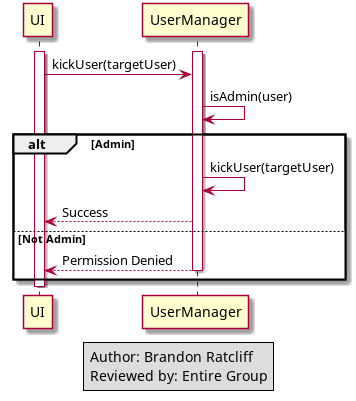
\includegraphics[width=\textwidth]{images/SequenceDiagrams/ProjectUserManagementKickUser}
\newpage

\subsubsection[Project User Management Feature 3: Set User Permissions Use Case Description ]{\selectlanguage{english}\rmfamily\bfseries\color{black}
	Project User Management Feature 3: Set User Permissions Use Case Description}
\hypertarget{RefHeading22059017292}{}

\vspace{2pt}
\hrule
\vspace{8pt}
 \textbf{Actors:} User \newline
\textbf{Goals:} Modify a user\'s permissions. \newline
 \textbf{Pre-conditions:} User has admin permissions, and the user whose permissions they wish to change is a member of the project\newline
 \textbf{Summary:} User modifies another User\'s permissions to the project. \newline
 \textbf{Related use cases:} None. \newline
\textbf{Steps:} \begin{enumerate}
  \item User clicks Permissions Management button.
  \item System displays permissions management window.
  \item User selects the user whose permissions they want to edit.
  \item System displays a list of toggles for the users's permissions.
  \item User makes changes to the user's permissions.
  \item System modifes the target User\'s permissions.
 \end{enumerate}
 \textbf{Alternatives:} None. \newline
 \textbf{Post-conditions:} None. \newline
\begin{itemize}
	\item \textbf{User}
	\item \textbf{Project}
	\item \textbf{UserManager}
	\item \textbf{Permissions}
\end{itemize}
\vspace{8pt}
\hrule
\newpage

\subsubsection[Project User Management Feature 3: Set User Permissions Sequence Diagram]{\selectlanguage{english}\rmfamily\bfseries\color{black}
	Project User Management Feature 3: Set User Permissions Sequence Diagram}
\hypertarget{RefHeading22059017292}{}
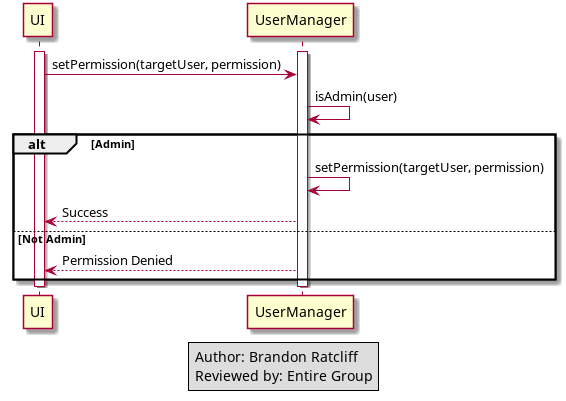
\includegraphics[width=\textwidth]{images/SequenceDiagrams/ProjectUserManagementSetPermission}
\newpage




{\selectlanguage{english}\color{black}
	\foreignlanguage{english}{\textit{For each feature, you should either provide a Use Case Description
		}}\foreignlanguage{english}{\textbf{\textit{or}}}\foreignlanguage{english}{\textit{ a Non-task feature description,
		whichever is more appropriate.}}}
\newpage

\subsection[Class Diagrams]{\selectlanguage{english}\rmfamily\bfseries\color{black} CLASS DIAGRAMS}
\hypertarget{RefHeading21659017292}{}{\selectlanguage{english}\color{black}

\subsubsection[Class Diagram 1: File Management]{\selectlanguage{english}\rmfamily\bfseries\color{black}
	Class Diagram 1: File Management}
\hypertarget{RefHeading22059017292}{}
\bigskip

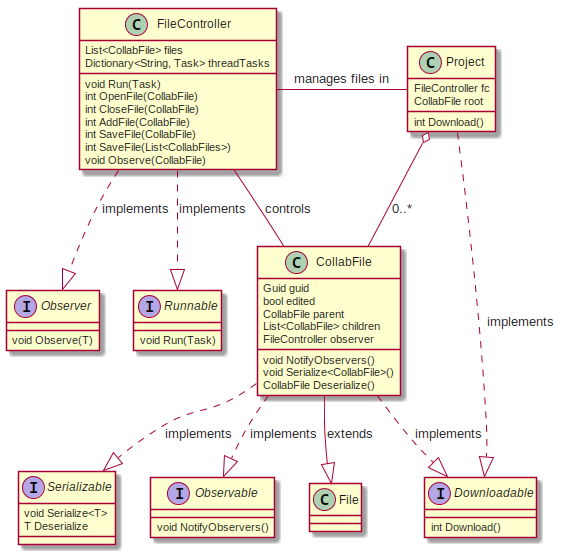
\includegraphics[width=\textwidth]{images/ClassDiagrams/FileManagement}

\newpage

\subsubsection[Class Diagram Description 1: File Management Description]{\selectlanguage{english}\rmfamily\bfseries\color{black}
	Class Diagram Description 1: File Management Description}
\hypertarget{RefHeading22059017292}{}

\textbf{Interfaces:}\\
\begin{itemize}
	\item The \textit{Observer} interface requires its implementers to implement a method with the following signature: \textbf{void Observe(T)}. The purpose of this method is for classes to implement ways in which to observe other classes. We foresee the \textbf{FileController} class implementing this interface in order to observe changes in \textbf{CollabFile} objects.
	\item The \textit{Runnable} interface requires its implementers to implement a method with the following signature: \textbf{void Run(Task)} where \textbf{Task} is a method that can be run in a separate thread. The \textbf{FileController} class will implement this interface in order to execute its IO operations in a separate thread. This will keep the UI thread free and our program responsive.
	\item The \textit{Serializable} interface requires its implementers to implement the \textbf{void Serialize<T>()} method and serializes objects of type \textbf{T}. It also requires the implementation of the \textbf{T Deserialize<T>()} method which will operate on a serialized string object and return an instantiated object of type \textbf{T}.
	\item The \textit{Observable} interface requires its implementers to have a list of observers and a method to notify its observers of changes to itself. The purpose of this implementation is to communicate with the \textbf{FileController} object and notify it when a CollabFile changes.
	\item The \textit{Downloadable} interface requires its implementers to implement a method with the following signature: \textbf{int Download()}. The purpose of this method is for classes to implement ways in which their objects can be downloaded. The \textbf{int} return type will be used as a status code. We foresee this interface being used with the \textbf{Project} and \textbf{CollabFile} classes, as the diagram shows, allowing users to download files or projects with the \textbf{Download()} method.
\end{itemize}
\textbf{Classes:}
\begin{itemize}
	\item The \textbf{FileController} class will manage the \textbf{CollabFile} objects in the \textbf{Project} class. It will do so by storing a list of files and a dictionary of its methods that can be run in a separate thread. Its methods all deal with managing files. It will implement the \textit{Observer} and \textit{Runnable} interfaces. Refer to the interfaces list above to see the details of such implementations.
	\item The \textbf{Project} class represents the entire project that users work on. This includes users, files, permissions, etc. For the sake of simplicity, this diagram only lists properties and methods relating to file editing. Objects of type \textbf{Project} will have a \textbf{FileController} and a root \textbf{CollabFile} as per a file-tree structure. The \textbf{Project} class must also implement the \textit{Downloadable} interface in order to specify how projects are downloaded.Refer to the interfaces list above to see the details of this implementation.
	\item the \textbf{CollabFile} class represents a file in a \textbf{Project}. It extends the \textbf{File} class for the purposes of allowing collaborative editing, among other project functions. It implements the \textit{Serializable} interface to allow its information to be transported over the internet in the best possible format. This requires the implementation of the \textbf{void Serialize<T>()} and \textbf{T Deserialize<SerializedString>()} methods which will handle serialization and deserialization. This class also implements the \textit{Observable} interface which will specify how it communicates with the \textbf{FileController} class in order to notify of relevant changes to \textbf{CollabFile} objects. This requires the implementation of a list of observers and a method to notify observers. Lastly, it implements the \textit{Downlodable} interface which will specify how \textbf{CollabFile} objects are to be downloaded. Refer to the interfaces list above for more details of such implementations.
\end{itemize}

\subsubsection[Class Diagram 2: File Editing]{\selectlanguage{english}\rmfamily\bfseries\color{black}
	Class Diagram 2: File Editing}
\hypertarget{RefHeading22059017292}{}
\bigskip

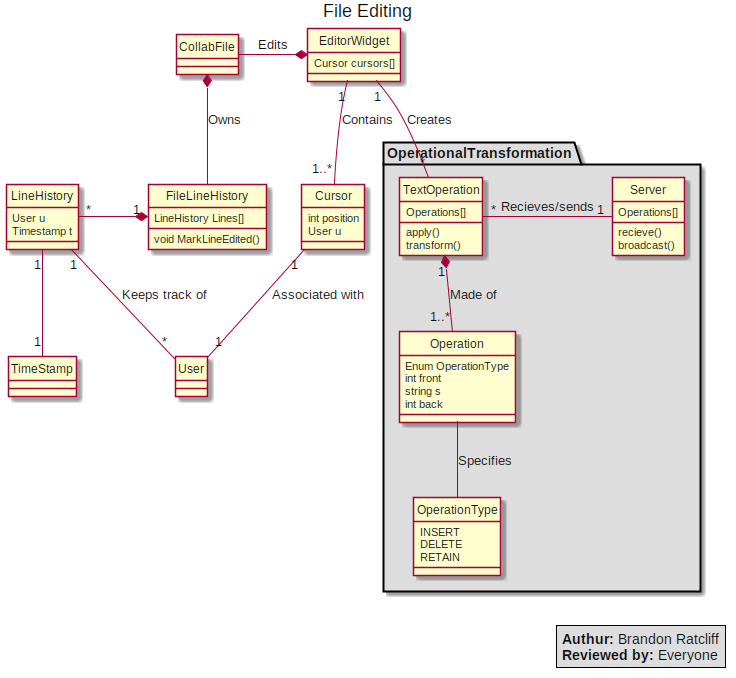
\includegraphics[width=\textwidth]{images/ClassDiagrams/EditFile}

\newpage

\subsubsection[Class Diagram Description 2: File Editing Description]{\selectlanguage{english}\rmfamily\bfseries\color{black}
	Class Diagram Description 2: File Editing Description}
\hypertarget{RefHeading22059017292}{}

\textbf{Editor:}\\
\begin{itemize}
\item The \textit{CollabFile} class is a class used in many of the other class diagrams in this project. It is the general class containing all the methods and variables for managing a file. It contains a \textbf{FileLineHistory} object. CollabFile has a list of \textbf{Cursor} objects, one for every user editing the file..
  \item The \textit{User} class is a class used in many of the class diagrams. It represents a single user of the sQuire program.
  \item The \textit{TimeStamp} class is used in several other places. It represents a date and time.
	\item The \textit{FileLineHistory} class is a class that keeps track of who last edited every line in the file. This will be used to display the changes inside the editor. It does this by having an array (one element per line in the file) of \textbf{LineHistory} objects.
  \item The \textit{LineHistory} class is contains the information used by the \textbf{FileLineHistory} class. It contains a \textbf{User} {the last one to edit a particular line} and a \textbf{Timestamp} (when the line was last edited). More fields can easily be added to this if it turns out there is more information we'd like to keep track of on a line-by-line basis.
	\item The \textit{EditorWidget} class is something that we will (hopefully) not write ourselves. It will be the editor widget we use for providing the code editor. Preliminary research found RSyntaxtTextArea (https://github.com/bobbylight/RSyntaxTextArea). This looks like a good fit because it has syntax highlighting, auto completion, code analysis, and of course, support from java. It also has a simple plugin architecture, so it looks like it would be easy to extend to our needs. More research needs to be done to figure out the exact class structure for this.
  \item The \textit{Cursor} class is made up of a \textbf{User} and a position within a file- everything that is needed to display a users cursor inside the editor.
\end{itemize}
\textbf{OperationalTransform:} \\\bigskip
I organized this one into a separate package because that's how I'm pretty sure we'll write it. The OperationalTransform algorithm is a collaborative editing algorithm used to allow multiple people to edit the same document at the same time, and keep the documents in sync. Ideally, we would use a pre-built library for this, as the algorithm is quite complex and there are lots of special cases, but I was unable to find one written in Java. Our best best will probably be to port an existing library in another language. The clearest, best documented implementation I found was OT.js (https://github.com/Operational-Transformation/ot.js/). The following classes are the main data structures implemented by this version of Operational Transformation.
\begin{itemize}
\item The \textit{TextOperation} class represents a sequence of \textbf{Operation} objects, or changes. The TextOperation can then be applied to a string, or transformed with anther TextOperation (from another client) in order account for changes that occurred simultaneously. See the Operational Transformation algorithm for more details.
\item The \textit{Operation} class represents a specific operation. This contains an \textbf{OperationType}, a integer front, which specifies the number of characters before the change, a string s, which contains the actual character changed (ex, inserted or deleted). And then an integer back, which contains the number of characters until the end of the document.
\item The \textit{OperationType} Enum is used to specify what type of operation a \textbf{Operation} is. Type can be either an INSERT, when character(s) are inserted to a document, DELETE, when character(s) are deleted from a document, or RETAIN, used to shift other operations.
\item the \textit{Server} class is a class that will be running on the server to sync changes between clients. It's job it to listen for \textbf{TextOperations} from all connected clients, and when it receives one, broadcast that change to all connected clients.
\end{itemize}
\newpage
\subsubsection[Class Diagram 3: Authentication]{\selectlanguage{english}\rmfamily\bfseries\color{black}
	Class Diagram 3: Authentication}
\hypertarget{RefHeading22059017292}{}
\bigskip

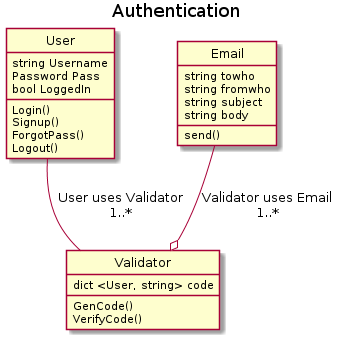
\includegraphics[width=\textwidth]{images/ClassDiagrams/Authentication}

\newpage

\subsubsection[Class Diagram Description 3: Authentication Description]{\selectlanguage{english}\rmfamily\bfseries\color{black}
	Class Diagram Description 3: Authentication Description}
\hypertarget{RefHeading22059017292}{}

\textbf{Classes:}
\begin{itemize}

	\item The \textbf{User} class represents the main user of the entire program. It details the basic information of each individual user, and allows each user the ability to create an account, to log into an existing account, and once logged in, to log out of the user account. It also allows a user to change his/her password, which involves the other classes.
	\item The \textbf{Email} class allows the program to send emails to Users who have signed up, or are signing up. It stores User information as a series of strings to be used by the \textbf{send()} function, which sends validation codes to Users' email addresses.
	\item The \textbf{Validator} class will run validation functions when called to do so by the User. Upon a User indicating they would like to change/have forgotten their password, it generates a validation code for that particular User, which it then stores in a dictionary. This validation code is sent to Users by means of the \textbf{send()} function denoted earlier.
\end{itemize}

\newpage

\subsubsection[Class Diagram 4: User Preferences]{\selectlanguage{english}\rmfamily\bfseries\color{black}
	Class Diagram 4: User Preferences}
\hypertarget{RefHeading22059017292}{}
\bigskip

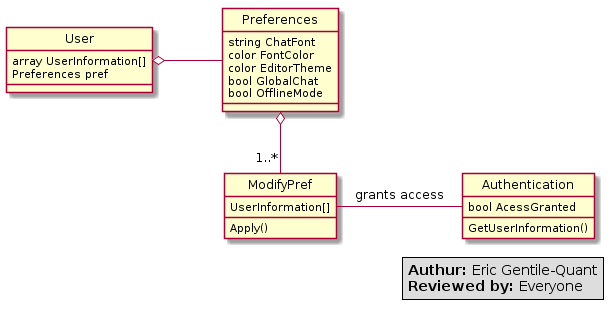
\includegraphics[width=\textwidth]{images/ClassDiagrams/UserPref}

\newpage

\subsubsection[Class Diagram Description 4: User Preferences Description]{\selectlanguage{english}\rmfamily\bfseries\color{black}
	Class Diagram Description 4: User Preferences Description}
\hypertarget{RefHeading22059017292}{}

\textbf{Classes:}
\begin{itemize}

       \item \textbf{User:} Represents the human user of the program. It will hold the user's profile information so that it can be validated later.
       \item \textbf{Preferences:} Holds all the user's account preferences. This includes profile picture, chat font, chat color, ect.
       \item \textbf{ModifyPref:} Allows the user to modify his or her's preferences.
       \item \textbf{Authentication:} Authenticates the user's username and password to allow access to make changes on their account.
\end{itemize}

\newpage
\subsubsection[Class Diagram 5: Communication]{\selectlanguage{english}\rmfamily\bfseries\color{black}
	Class Diagram 5: Communication}
\hypertarget{RefHeading22059017292}{}
\bigskip

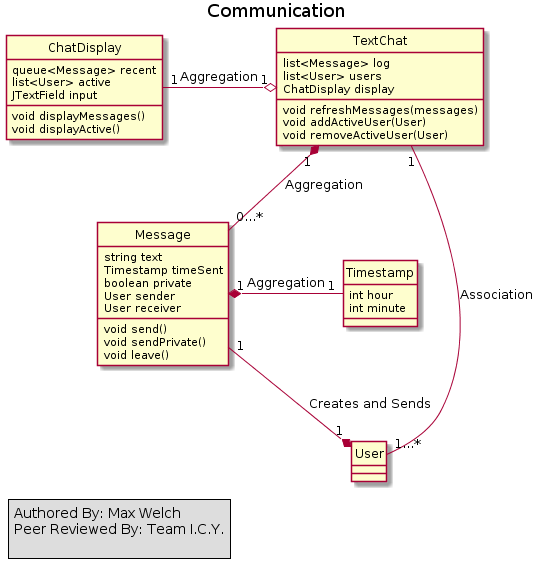
\includegraphics[width=\textwidth]{images/ClassDiagrams/Communication}

\newpage
\subsubsection[Class Diagram Description 5: Communication Description]{\selectlanguage{english}\rmfamily\bfseries\color{black}
	Class Diagram Description 5: Communication Description}
\hypertarget{RefHeading22059017292}{}

\textbf{Classes:}
\begin{itemize}

	\item \textbf{TextChat:} The master class to manage the messages, users, and display of the system.
	\item \textbf{ChatDisplay:} Displays relevant information including most recent 20 messages and active users
	\item \textbf{User:} Users interacting with the chat system.
	\item \textbf{Message:} Messages sent by users to TextChat, contain a string, timestamp, and sender/receiver data.
	\item \textbf{Timestamp:} Recorded time of when message was sent.
\end{itemize}
\newpage

\subsubsection[Class Diagram 6: Project Browsing]{\selectlanguage{english}\rmfamily\bfseries\color{black}
	Class Diagram 6: Project Browsing}
\hypertarget{RefHeading22059017292}{}
\bigskip

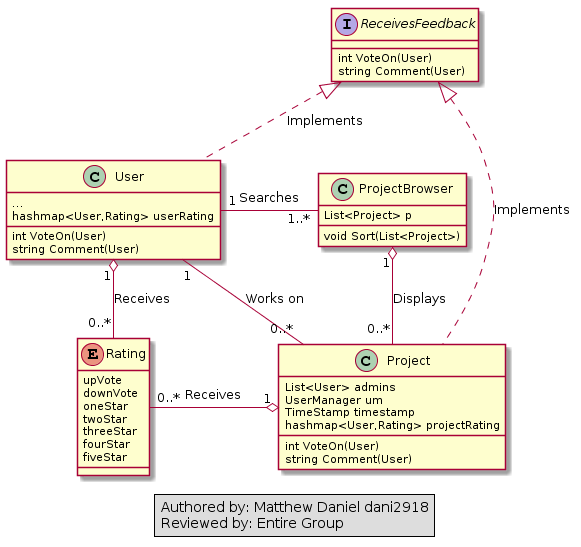
\includegraphics[width=\textwidth]{images/ClassDiagrams/ProjectBrowsing}

\newpage

\subsubsection[Class Diagram Description 6: Project Browsing]{\selectlanguage{english}\rmfamily\bfseries\color{black}
	Class Diagram Description 6: Project Browsing}
\hypertarget{RefHeading22059017292}{}


\textbf{Enums:}\\
\begin{itemize}
	\item The \textit{Rating} enum produces a value based upon the user's desired rating of another user or a project.
\end{itemize}
\textbf{Interfaces:}\\
\begin{itemize}
	\item The \textit{Receives Feedback} interface requires its implementers to implement two methods: \textbf{int VoteOnUser(User)}, which returns a value based on a user's rating, and \textbf{string Comment(User)}, which leaves feedback in the form of a comment.
\end{itemize}
\textbf{Classes:}
\begin{itemize}
	\item The \textbf{User} class will be the class, shared across many of the class diagrams, that stores information about a user. The User class will have not only the methods and fields shown in this diagram, but a concatenation of the ones shown here and all other methods and fields from the other diagrams. Here, the User class implements the ReceivesFeedback interface so that other users may leave comments/reviews of a User object, and so that they may receive an accompanying rating from one to five stars. In relation to browsing projects, a User is the agent who searches a ProjectBrower object and works on a Project object.
	\item The \textbf{Project} class will also have the methods and fields of other class diagrams, similar to the User class above. Here, the Project class implements the ReceivesFeedback interface so that users may leave comments/reviews on projects, as well as vote up or down on projects that they come across. Projects are displayed in the ProjectBroswer class and worked on by users.
	\item The \textbf{ProjectBrowser} class contains a search-able list of zero or more projects tailored to a user's search. Users browse the list in order to find projects of interest.
\end{itemize}

\newpage
\subsubsection[Class Diagram 7: Project User Management]{\selectlanguage{english}\rmfamily\bfseries\color{black}
	Class Diagram 7: Project User Management}
\hypertarget{RefHeading22059017292}{}
\bigskip

\includegraphics[width=\textwidth]{images/ClassDiagrams/ProjectUserManagement}

\newpage

\subsubsection[Class Diagram Description 7: Project User Management Description]{\selectlanguage{english}\rmfamily\bfseries\color{black}
	Class Diagram Description 7: Project User Management Description}
\hypertarget{RefHeading22059017292}{}

\textbf{Classes:}
\begin{itemize}

	\item The \textbf{User} class contains the profiles of everyone who uses sQuire, and identifies anyone who tries to access a board.
	\item The \textbf{Project} class contains all of the information pertinent to an individual project, including one UserManager, which the client uses to control what kind of access each user has to that specific project.
	\item The \textbf{UserManager} class is referenced to check if a user has permission to read, modify, or run a project, or invite, ban, or change the permissions of another user. It does this by updating and checking against a HashMap of Permissions idexed by User. It records the User profile of the project creator to prevent the creator being demoted by another admin. It also contains a set of Permissions to use by default, before users are manually added to the project.
	The functions AddUser, KickUser, and SetPerms all modify the permissions HashMap after checking against it to make sure the active user has the authority to change the permissions of the target user.
	\item The \textbf{HashMap} class, in this case, functions as a permissions lookup table. It's indexed by User, and for each User in it there's one set of Permissions that it returns.
	\item The \textbf{Permissions} class is a set of bools that store whether each User has permission (within the instance's parent project) to read, write, execute the project, invite users, and/or modify the permissions of other users regarding the project.
\end{itemize}

\newpage

\subsubsection[Class Diagram 8: Project Management]{\selectlanguage{english}\rmfamily\bfseries\color{black}
	Class Diagram 8: Project Management}
\hypertarget{RefHeading22059017292}{}
\bigskip

\includegraphics[width=\textwidth]{images/ClassDiagrams/ProjectManagement}

\subparagraph[]{\selectlanguage{english}\rmfamily\color{black} }
\clearpage\setcounter{page}{1}\pagestyle{Convertvi}
\section[REQUIREMENTS TRACEABILITY]{\selectlanguage{english}\rmfamily\bfseries\color{black} REQUIREMENTS TRACEABILITY}
\hypertarget{RefHeading28459017292}{}{\selectlanguage{english}\itshape\color{black}
This section shall contain traceability information from each system requirement in this specification to the system (or
subsystem, if applicable) requirements it addresses. \ A tabular form is preferred, but not mandatory.}


\bigskip


\begin{flushleft}
\tablefirsthead{\hline
\multicolumn{1}{|m{0.9212598in}|}{\centering{\selectlanguage{english}\bfseries\color{black} Feature Name}} &
\centering{\selectlanguage{english}\bfseries\color{black} Req No.} &
\centering{\selectlanguage{english}\bfseries\color{black} Requirement Description} &
\centering{\selectlanguage{english}\bfseries\color{black} Priority} &
\centering{\selectlanguage{english}\bfseries\color{black} SDD} &
\multicolumn{2}{m{1.2872598in}|}{\centering{\selectlanguage{english}\bfseries\color{black} Alpha Release}} &
\multicolumn{2}{m{1.3587599in}|}{\centering{\selectlanguage{english}\bfseries\color{black} Beta Release}} &
\multicolumn{2}{m{1.3795599in}|}{\centering{\selectlanguage{english}\bfseries\color{black} Final Test}}\\\hline
 &
 &
 &
 &
 &
\centering{\selectlanguage{english}\bfseries\color{black} Test Case(s)} &
\centering{\selectlanguage{english}\bfseries\color{black} Test Res.} &
\centering{\selectlanguage{english}\bfseries\color{black} Test Case(s)} &
\centering{\selectlanguage{english}\bfseries\color{black} Test Res.} &
\centering{\selectlanguage{english}\bfseries\color{black} Test Case(s)} &
{\selectlanguage{english}\bfseries\color{black} Test Res.}\\}
\tablehead{\hline
\multicolumn{1}{|m{0.9212598in}|}{\centering{\selectlanguage{english}\bfseries\color{black} Feature Name}} &
\centering{\selectlanguage{english}\bfseries\color{black} Req No.} &
\centering{\selectlanguage{english}\bfseries\color{black} Requirement Description} &
\centering{\selectlanguage{english}\bfseries\color{black} Priority} &
\centering{\selectlanguage{english}\bfseries\color{black} SDD} &
\multicolumn{2}{m{1.2872598in}|}{\centering{\selectlanguage{english}\bfseries\color{black} Alpha Release}} &
\multicolumn{2}{m{1.3587599in}|}{\centering{\selectlanguage{english}\bfseries\color{black} Beta Release}} &
\multicolumn{2}{m{1.3795599in}|}{\centering{\selectlanguage{english}\bfseries\color{black} Final Test}}\\\hline
 &
 &
 &
 &
 &
\centering{\selectlanguage{english}\bfseries\color{black} Test Case(s)} &
\centering{\selectlanguage{english}\bfseries\color{black} Test Res.} &
\centering{\selectlanguage{english}\bfseries\color{black} Test Case(s)} &
\centering{\selectlanguage{english}\bfseries\color{black} Test Res.} &
\centering{\selectlanguage{english}\bfseries\color{black} Test Case(s)} &
{\selectlanguage{english}\bfseries\color{black} Test Res.}\\}
\tabletail{}
\tablelasttail{}
\begin{supertabular}{m{0.9212598in}|m{0.42125985in}|m{1.9212599in}|m{0.39275986in}|m{0.7587598in}|m{0.6622598in}|m{0.5462598in}|m{0.6712598in}|m{0.6087598in}|m{0.6712598in}|m{0.6295598in}|}
\hhline{~~~~~------}
\multicolumn{1}{|m{0.9212598in}|}{~
} &
\centering{\selectlanguage{english}\color{black} 1.1} &
~
 &
~
 &
~
 &
~
 &
~
 &
~
 &
~
 &
~
 &
~
\\\hline
 &
\centering{\selectlanguage{english}\color{black} 1.2} &
~
 &
~
 &
~
 &
~
 &
~
 &
~
 &
~
 &
~
 &
~
\\\hhline{~----------}
 &
\centering{\selectlanguage{english}\color{black} {\dots}} &
~
 &
~
 &
~
 &
~
 &
~
 &
~
 &
~
 &
~
 &
~
\\\hhline{~----------}
 &
\centering{\selectlanguage{english}\color{black} 1.[n]} &
~
 &
~
 &
~
 &
~
 &
~
 &
~
 &
~
 &
~
 &
~
\\\hhline{~----------}
\multicolumn{1}{|m{0.9212598in}|}{~
} &
\centering{\selectlanguage{english}\color{black} 2.1} &
~
 &
~
 &
~
 &
~
 &
~
 &
~
 &
~
 &
~
 &
~
\\\hline
 &
\centering{\selectlanguage{english}\color{black} 2.2} &
~
 &
~
 &
~
 &
~
 &
~
 &
~
 &
~
 &
~
 &
~
\\\hhline{~----------}
 &
\centering{\selectlanguage{english}\color{black} {\dots}} &
~
 &
~
 &
~
 &
~
 &
~
 &
~
 &
~
 &
~
 &
~
\\\hhline{~----------}
 &
\centering{\selectlanguage{english}\color{black} 2.[n]} &
~
 &
~
 &
~
 &
~
 &
~
 &
~
 &
~
 &
~
 &
~
\\\hhline{~----------}
\multicolumn{1}{|m{0.9212598in}|}{~
} &
\centering{\selectlanguage{english}\color{black} 3.1} &
~
 &
~
 &
~
 &
~
 &
~
 &
~
 &
~
 &
~
 &
~
\\\hline
 &
\centering{\selectlanguage{english}\color{black} 3.2} &
~
 &
~
 &
~
 &
~
 &
~
 &
~
 &
~
 &
~
 &
~
\\\hhline{~----------}
 &
\centering{\selectlanguage{english}\color{black} {\dots}} &
~
 &
~
 &
~
 &
~
 &
~
 &
~
 &
~
 &
~
 &
~
\\\hhline{~----------}
 &
\centering{\selectlanguage{english}\color{black} 3.[n]} &
~
 &
~
 &
~
 &
~
 &
~
 &
~
 &
~
 &
~
 &
~
\\\hhline{~----------}
\multicolumn{1}{|m{0.9212598in}|}{{\selectlanguage{english}\color{black} {\dots}}} &
\centering{\selectlanguage{english}\color{black} {\dots}} &
~
 &
~
 &
~
 &
~
 &
~
 &
~
 &
~
 &
~
 &
~
\\\hline
\multicolumn{1}{|m{0.9212598in}|}{~
} &
\centering{\selectlanguage{english}\color{black} [m].1} &
~
 &
~
 &
~
 &
~
 &
~
 &
~
 &
~
 &
~
 &
~
\\\hline
 &
\centering{\selectlanguage{english}\color{black} [m].2} &
~
 &
~
 &
~
 &
~
 &
~
 &
~
 &
~
 &
~
 &
~
\\\hhline{~----------}
\multicolumn{1}{|m{0.9212598in}|}{~
} &
\centering{\selectlanguage{english}\color{black} {\dots}} &
~
 &
~
 &
~
 &
~
 &
~
 &
~
 &
~
 &
~
 &
~
\\\hline
\multicolumn{1}{|m{0.9212598in}|}{~
} &
\centering{\selectlanguage{english}\color{black} [m.n]} &
~
 &
~
 &
~
 &
~
 &
~
 &
~
 &
~
 &
~
 &
~
\\\hline
\end{supertabular}
\end{flushleft}
{\selectlanguage{english}\color{black}
Priorities are: \textbf{M}andatory, \textbf{L}ow, \textbf{H}igh}

{\selectlanguage{english}\color{black}
SDD link is version and page number or function name.}

{\selectlanguage{english}\color{black}
Test cases and results are file names and \textbf{P}ass/\textbf{F}ail or \% passing.}

\clearpage\setcounter{page}{1}\pagestyle{Convertvii}
\section[APPENDIX A. \ [insert name here{]}]{\selectlanguage{english}\rmfamily\bfseries\color{black} APPENDIX A.
\ [insert name here]}
\hypertarget{RefHeading28659017292}{}
\bigskip

{\selectlanguage{english}\itshape\color{black}
Include copies of specifications, mockups, prototypes, etc. supplied or derived from the customer. \ Appendices are
labeled A, B, {\dots}n. \ \ Reference each appendix as appropriate in the text of the document. }

{\selectlanguage{english}\color{black}
\foreignlanguage{english}{\ [ insert appendix A here ]}}

\clearpage\setcounter{page}{1}\pagestyle{Convertviii}
\section[APPENDIX B. \ [insert name here{]}]{\selectlanguage{english}\rmfamily\bfseries\color{black} APPENDIX B.
\ [insert name here]}
\hypertarget{RefHeading28859017292}{}
\bigskip

{\selectlanguage{english}\color{black}
[ insert appendix B here ]}


\bigskip
\end{document}
